\documentclass[12pt,a4paper]{report}

% ===== PRÉAMBULE =====
% ========================================
% PACKAGES DE BASE
% ========================================
\usepackage[utf8]{inputenc}                    % Encodage UTF-8 pour les caractères accentués
\usepackage[T1]{fontenc}                       % Encodage de sortie pour les polices européennes
\usepackage[french]{babel}                     % Support de la langue française

% ========================================
% PACKAGES MATHÉMATIQUES
% ========================================
\usepackage{mathtools}                         % Extension d'amsmath avec outils supplémentaires
\usepackage{amsfonts}                          % Polices mathématiques AMS
\usepackage{amssymb}                           % Symboles mathématiques AMS
\usepackage{amsthm}                            % Environnements de théorèmes
\usepackage{mathrsfs}                          % Lettres calligraphiques \mathscr{}

% ========================================
% PACKAGES GRAPHIQUES ET COULEURS
% ========================================
\usepackage{graphicx}                          % Inclusion et manipulation d'images
\usepackage[dvipsnames]{xcolor}                % Couleurs étendues (noms prédéfinis)
\usepackage{tikz}                              % Graphiques TikZ
\usepackage{tikz-cd}                           % Diagrammes commutatifs
\usetikzlibrary{calc}

% ========================================
% PACKAGES DE MISE EN PAGE
% ========================================
\usepackage[a4paper, margin=1in]{geometry}    % Configuration des marges
\usepackage{fancyhdr}                          % En-têtes et pieds de page personnalisés
\usepackage{titlesec}                          % Personnalisation des titres de sections
\usepackage{setspace}                          % Contrôle de l'interligne
\usepackage{titling} %Récupération du nom des auteurs                            
% Configuration détaillée des marges
\geometry{
    top=2.5cm,
    bottom=2.5cm,
    left=2.5cm,
    right=2.5cm,
    headheight=15.03pt,
    headsep=20pt,
    footskip=30pt
}

% ========================================
% PACKAGES DE MISE EN FORME
% ========================================
\usepackage{textcomp}                          % Symboles textuels supplémentaires
\usepackage{soul}                              % Soulignement et surlignage avancés
\usepackage{mdframed}                          % Boîtes encadrées personnalisables
\usepackage{tcolorbox}                         % Boîtes colorées avancées

% ========================================
% LISTES ET ÉNUMÉRATIONS
% ========================================
\usepackage[shortlabels]{enumitem}
\setlistdepth{9}
\renewlist{enumerate}{enumerate}{9}
\renewlist{itemize}{itemize}{9}

% Configuration des niveaux d'énumération
\setlist[enumerate,1]{label=(\roman*)}
\setlist[enumerate,2]{label=(\alph*)}
\setlist[enumerate,3]{label=\arabic*.}
\setlist[enumerate,4]{label=(\roman*)}
\setlist[enumerate,5]{label=(\alph*)}

% Configuration des niveaux d'itemize
\setlist[itemize,1]{label=$\bullet$}
\setlist[itemize,2]{label=$\circ$}
\setlist[itemize,3]{label=$-$}
\setlist[itemize,4]{label=$\ast$}

% ========================================
% HYPERLIENS
% ========================================
\definecolor{linkcolor}{RGB}{0,0,139}
\definecolor{citecolor}{RGB}{139,0,0}
\definecolor{urlcolor}{RGB}{0,100,0}

\usepackage[
    colorlinks=true,
    linkcolor=linkcolor,
    citecolor=citecolor,
    urlcolor=urlcolor,
    bookmarks=true,
    bookmarksnumbered=true,
    pdfstartview=FitH
]{hyperref}

% ========================================
% POLICES MATHÉMATIQUES
% ========================================
\usepackage{fouriernc}                         % Police Fourier
\DeclareMathAlphabet{\mathbb}{U}{msb}{m}{n}    % \mathbb standard (AMS)
\DeclareMathAlphabet{\mathcal}{OMS}{cmsy}{m}{n} % \mathcal standard

% ========================================
% STYLES POUR LES BOÎTES
% ========================================
\definecolor{lime}{RGB}{0,0,128}

% Macro pour définir des styles rapidement
\newcommand{\defstyle}[2]{\mdfdefinestyle{#1}{
    leftmargin=0pt,
    rightmargin=0pt,
    innerleftmargin=10pt,
    innerrightmargin=10pt,
    innertopmargin=0pt,
    innerbottommargin=2pt,
    leftline=true,
    rightline=false,
    topline=false,
    bottomline=false,
    linecolor=#2,
    linewidth=2pt,
    backgroundcolor=white
}}

% Styles spécifiques
\defstyle{definitionstyle}{RoyalBlue}
\defstyle{theoremstyle}{lime}
\defstyle{attentionstyle}{Red}

% Style classique (sans bordure colorée)
\mdfdefinestyle{classicstyle}{
    leftmargin=0pt,
    rightmargin=0pt,
    innerleftmargin=0pt,
    innerrightmargin=0pt,
    innertopmargin=0pt,
    innerbottommargin=2pt,
    leftline=true,
    rightline=false,
    topline=false,
    bottomline=false,
    linecolor=white,
    linewidth=2pt,
    backgroundcolor=white
}

% ========================================
% ENVIRONNEMENTS DE THÉORÈMES
% ========================================

% Définitions et axiomes
\newmdtheoremenv[style=definitionstyle,nobreak=true]{definition}{Définition}[section]
\newmdtheoremenv[style=definitionstyle,nobreak=true]{axiome}[definition]{Axiome}
\newmdtheoremenv[style=definitionstyle,nobreak=true]{conjecture}[definition]{Conjecture}
\newmdtheoremenv[style=definitionstyle,nobreak=true]{convention}[definition]{Convention}

% Théorèmes et résultats
\newmdtheoremenv[style=theoremstyle,nobreak=true]{theoreme}[definition]{Théorème}
\newmdtheoremenv[style=theoremstyle,nobreak=true]{lemme}[definition]{Lemme}
\newmdtheoremenv[style=theoremstyle,nobreak=true]{proposition}[definition]{Proposition}
\newmdtheoremenv[style=theoremstyle,nobreak=true]{corollaire}[definition]{Corollaire}

% Style amsthm
\newtheoremstyle{remarkstyle}
  {}{}
  {\normalfont}  % corps en droit
  {}
  {\itshape\bfseries}     % titre en italique
  {.}{ }{}

% Environnements auxiliaires
\theoremstyle{remarkstyle}


\newtheorem{remarque}[definition]{Remarque}
\surroundwithmdframed[style=classicstyle]{remarque}
% Style amsthm
\newtheoremstyle{normalstyle}
  {}{}
  {\normalfont}  % corps en droit
  {}
  {\normalfont\bfseries}     % titre en italique
  {.}{ }{}

% Environnements auxiliaires
\theoremstyle{normalstyle}
\newtheorem{exercice}[definition]{Exercice}
\surroundwithmdframed[style=classicstyle]{exercice}
\newtheorem{exemple}[definition]{Exemple}
\surroundwithmdframed[style=classicstyle]{exemple}
\newtheorem*{resolution}{Résolution}
\surroundwithmdframed[style=classicstyle]{resolution}
\newtheorem*{notation}{Notation}
\surroundwithmdframed[style=classicstyle]{notation}

% ========================================
% EN-TÊTES ET PIEDS DE PAGE
% ========================================
\pagestyle{fancy}
\fancyhf{}
\fancyhead[L]{\textit{\leftmark}}              % Chapitre à gauche
\fancyfoot[L]{\thepage}                        % Numéro de page à gauche
\fancyfoot[R]{\textit{\rightmark}}             % Section à droite

\renewcommand{\headrulewidth}{0pt}
\renewcommand{\footrulewidth}{0pt}

% Marques de chapitres et sections
\renewcommand{\chaptermark}[1]{%
    \markboth{\MakeUppercase{\chaptername\ \thechapter.\ #1}}{}}
\renewcommand{\sectionmark}[1]{%
    \markright{\MakeUppercase{\thesection.\ #1}}}

% Style pour les premières pages de chapitre
\fancypagestyle{plain}{%
    \fancyhf{}
    \fancyfoot[L]{\thepage}
    \fancyfoot[R]{\textit{\rightmark}}
}

% ========================================
% FORMAT DES TITRES DE SECTIONS
% ========================================
\titleformat{\chapter}[block]
    {\normalfont\LARGE\bfseries\scshape\color{RoyalBlue}\flushleft}
    {\thechapter.}
    {1em}
    {\scshape\color{RoyalBlue}}

\titleformat{\section}[block]
    {\normalfont\large\scshape\color{RoyalBlue}\flushleft}
    {\thesection}
    {1em}
    {}

\titleformat{\subsection}[block]
    {\normalfont\large\scshape\color{RoyalBlue}\flushleft}
    {\thesubsection}
    {1em}
    {}

\titleformat{\subsubsection}[block]
    {\normalfont\large\scshape\color{RoyalBlue}\flushleft}
    {\thesubsubsection}
    {1em}
    {}

% ========================================
% ENSEMBLES USUELS
% ========================================
\newcommand{\N}{\mathbb{N}}                    % Entiers naturels
\newcommand{\Z}{\mathbb{Z}}                    % Entiers relatifs
\newcommand{\Q}{\mathbb{Q}}                    % Rationnels
\newcommand{\R}{\mathbb{R}}                    % Réels
\newcommand{\C}{\mathbb{C}}                    % Complexes
\newcommand{\K}{\mathbb{K}}                    % Corps quelconque
\newcommand{\Sg}{\mathfrak{S}}                 % Groupe symétrique
\newcommand{\sn}{\mathbb{S}_n}                 % Sphère de dimension n

% ========================================
% LOGIQUE
% ========================================
\newcommand{\ssi}{\Leftrightarrow}             % Si et seulement si
\newcommand{\alors}{\Rightarrow}               % Implique
\newcommand{\si}{\Leftarrow}                   % Est impliqué par

% ========================================
% NORMES ET DISTANCES
% ========================================
\newcommand{\norm}[1]{\left\| #1 \right\|}     % Norme
\newcommand{\norme}[1]{\lVert #1 \rVert}       % Norme (variante)
\newcommand{\abs}[1]{\left| #1 \right|}        % Valeur absolue

% ========================================
% INTERVALLES
% ========================================
\newcommand{\interoo}[1]{\left] #1\right[}  % ]a,b[
\newcommand{\interof}[1]{\left] #1\right]}   % ]a,b]
\newcommand{\interfo}[1]{\left[ #1\right[}   % [a,b[
\newcommand{\interff}[1]{\left[ #1\right]}   % [a,b]

% ========================================
% TOPOLOGIE
% ========================================
\newcommand{\topologie}{\mathcal{T}}           % Topologie
\newcommand{\voisinage}{\mathcal{V}}           % Voisinages
\newcommand{\partie}{\mathscr{P}}              % Parties
\newcommand{\filtre}{\mathscr{F}}              % Filtre
\newcommand{\ouvert}{\mathcal{O}}              % Ouverts
\newcommand{\ferme}{\mathcal{F}}               % Fermés
\newcommand{\adh}{\operatorname{adh}}                % Adhérence
% ========================================
% FONCTIONS
% ========================================
\newcommand{\fonction}[3]{#1\colon \left\{\begin{array}{l}#2 \\#3\end{array}\right.}

% ========================================
% OPÉRATEURS MATHÉMATIQUES
% ========================================
\DeclareMathOperator{\dom}{dom}               % Domaine
\DeclareMathOperator{\im}{Im}                 % Image
\DeclareMathOperator{\e}{e}                   % Exponentielle
\DeclareMathOperator{\stab}{St}               % Stabilisateur
\DeclareMathOperator{\orb}{Orb}               % Orbite
\DeclareMathOperator{\coker}{coker}           % Conoyau
\DeclareMathOperator{\sgn}{sgn}               % Signature
\DeclareMathOperator{\Frac}{Frac}             % Corps des fractions
\DeclareMathOperator{\Eq}{Eq}                 % Égaliseur
\DeclareMathOperator{\Coeq}{Coeq}             % Coégaliseur
\DeclareMathOperator{\Cone}{Cone}             % Catégorie des cônes
\DeclareMathOperator{\colim}{colim}           % Colimite

% Limites avec indices
\newcommand{\limi}{\lim\limits}

% Intégrale différentielle
\newcommand{\intd}{\,\operatorname{d}}
\newcommand{\dpart}[2]{\frac{\partial #1}{\partial #2}}

% ========================================
% THÉORIE DES CATÉGORIES
% ========================================

% --- Catégories standards ---
\newcommand{\Set}{\mathbf{Set}}               % Ensembles
\newcommand{\Grp}{\mathbf{Grp}}               % Groupes
\newcommand{\Ab}{\mathbf{Ab}}                 % Groupes abéliens
\newcommand{\Ring}{\mathbf{Ring}}             % Anneaux
\newcommand{\CRing}{\mathbf{CRing}}           % Anneaux commutatifs
\newcommand{\Mod}{\mathbf{Mod}}               % Modules
\newcommand{\Vect}{\mathbf{Vect}}             % Espaces vectoriels
\newcommand{\Top}{\mathbf{Top}}               % Espaces topologiques
\newcommand{\Pos}{\mathbf{Pos}}               % Ensembles ordonnés
\newcommand{\Cat}{\mathbf{Cat}}               % Catégories
\newcommand{\Mon}{\mathbf{Mon}}               % Monoïdes

% --- Constructions ---
\newcommand{\Disc}{\mathbf{Disc}}             % Catégorie discrète
\newcommand{\op}{^{\mathrm{op}}}              % Catégorie opposée

% --- Objets et morphismes ---
\newcommand{\Ob}{\mathrm{Ob}}                 % Objets
\newcommand{\Hom}{\mathrm{Hom}}               % Morphismes
\newcommand{\End}{\mathrm{End}}               % Endomorphismes
\newcommand{\Aut}{\mathrm{Aut}}               % Automorphismes
\newcommand{\id}{\mathrm{id}}                 % Identité
\newcommand{\Id}{\mathrm{Id}}                 % Foncteur identité

% --- Groupes linéaires ---
\newcommand{\GL}{\mathrm{GL}}                 % Groupe linéaire général
\newcommand{\SL}{\mathrm{SL}}                 % Groupe spécial linéaire

% ========================================
% TOPOLOGIE ALGÉBRIQUE
% ========================================

% --- Espaces classiques ---
\newcommand{\Sph}[1]{S^{#1}}                  % Sphère S^n
\newcommand{\Boule}[1]{D^{#1}}                % Boule D^n
\newcommand{\Tore}{T^2}                        % Tore
\newcommand{\RP}[1]{\mathbb{RP}^{#1}}         % Espace projectif réel
\newcommand{\CP}[1]{\mathbb{CP}^{#1}}         % Espace projectif complexe
\newcommand{\simplex}{\Delta}                  % Simplexe standard

% --- Groupes d'homotopie ---
\newcommand{\pifond}[2]{\pi_1(#1,#2)}         % π₁(X,x₀)
\newcommand{\pihomo}[2]{\pi_{#1}(#2)}         % πₙ(X)

% --- Homologie et cohomologie ---
\newcommand{\Hsing}[1]{H_{#1}}                % Homologie H_n
\newcommand{\Cohsing}[1]{H^{#1}}              % Cohomologie H^n
\newcommand{\Htilde}[1]{\widetilde{H}_{#1}}   % Homologie réduite

% --- Complexes de chaînes ---
\newcommand{\Csing}[1]{C_{#1}}                % Chaînes singulières C_n
\newcommand{\Zsing}[1]{Z_{#1}}                % Cycles Z_n
\newcommand{\Bsing}[1]{B_{#1}}                % Bords B_n

% --- Relations ---
\newcommand{\iso}{\cong}                       % Isomorphisme
\newcommand{\rel}{\,\text{rel}\,}             % Relatif à

% ========================================
% NOTATIONS DIVERSES
% ========================================
\newcommand{\xn}{(x_n)_{n\in I}}              % Suite indexée par I
\newcommand{\yn}{(y_n)_{n\in J}}              % Suite indexée par J
%Pour la page de garde
\newcommand{\teacher}{Q.Menet}
\title{Calcul différentiel}
\author{Piette \and Hamiot \and Alex}
\newcommand{\grade}{BaB2}

\begin{document}

% =====PAGE DE GARDE=====
\definecolor{encre}{RGB}{28,28,30}
\definecolor{accent}{RGB}{90,110,140}
\begin{titlepage}
\thispagestyle{empty}

% ---------- Filigrane : le cercle d'Apollonius ----------
\begin{tikzpicture}[remember picture, overlay]
  \node[opacity=0.16] at ($(current page.center)+(0,-0.6cm)$)
    {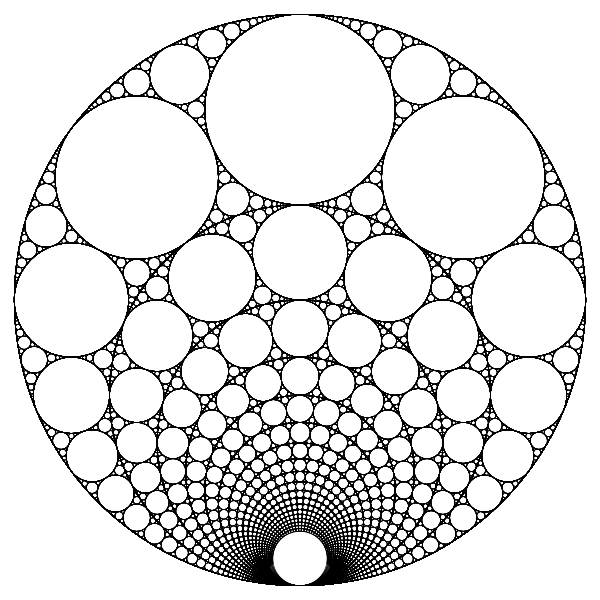
\includegraphics[width=17cm]{apollonius.png}};
\end{tikzpicture}

% ---------- Contenu ----------
\begin{center}
\vspace*{2.2cm}

{\footnotesize\color{accent}\scshape\selectfont
 \setlength{\baselineskip}{1.6em}
 Université de Mons \quad$\cdot$\quad Faculté des Sciences\par}

\vspace{3.4cm}

{\color{accent}\rule{2.2cm}{0.8pt}}

\vspace{1.1cm}

{\fontsize{43}{50}\selectfont\color{encre}
 Calcul Différentiel\par}

\vspace{1.0cm}

{\large\color{encre} Notes de cours\par}

\vspace{0.9cm}

{\color{accent}\rule{2.2cm}{0.8pt}}

\vfill

{\normalsize\color{encre}\scshape Tiago \& Hamiot \& Alex\par}
\vspace{0.35cm}
{\footnotesize\color{accent}BaB2 -- Sciences mathématiques\par}
\vspace{0.15cm}
{\footnotesize\color{accent}2026\,--\,2027\par}

\vspace{1.4cm}
\end{center}

\end{titlepage}


% ===== TABLE DES MATIÈRES =====
\tableofcontents
\newpage

% ===== CHAPITRES =====
\chapter{Espaces vectoriels normés}
En première année, nous avons étudié les réels, les suites de réels et les fonctions numériques. Un outil important est la valeur absolue. Elle permet d'évaluer la distance entre deux réels $x$ et $y$: $|x-y|$
\section{Distance}
\begin{definition}
    Soit $E$ un ensemble, une distance $d$ est une fonction de $E\times E$ dans $[0,+\infty[$ vérifiant :
    \begin{enumerate}
        \item $\forall x,y\in E \quad d(x,y)=0 \Leftrightarrow x=y$
        \item $\forall x,y\in E \quad d(x,y)=d(y,x)$
        \item $\forall x,y,z \in E \quad d(x,y)\leq d(x,z)+d(z,y)$
    \end{enumerate}
\end{definition}
\begin{exemple}
Sur $\mathbb{R}$, l'application $d(x,y)=|x-y|$ est une distance. Sur $E$ un ensemble non vide, l'application (distance discrète)
\[
d(x,y)=\begin{cases}
1 & \text{si } x \neq y, \\
0 & \text{si } x = y.
\end{cases}
\]
\end{exemple}
\section{Norme}
Si $E$ est un $\mathbb{K}$-espace vectoriel (avec $\mathbb{K}=\mathbb{R} \text{ ou } \mathbb{C}$) on aimerait que pour tous $x,y,z\in E$ et pour tout $\lambda\in \mathbb{K}$
\begin{enumerate}
    \item $d(x+z,y+z)=d(x,y)$ \quad (invariance par translation)
    \item $d(\lambda x,\lambda y)=\abs{\lambda}d(x,y)$ \quad (homogénéité absolue)
\end{enumerate}
Pour satisfaire ces conditions, on introduit la notion de norme.
\begin{definition}
    Soit $E$ un $\mathbb{K}-$espace vectoriel. Une norme $\lVert \cdot\rVert$ est une application de $E$ dans $[0,+\infty[$ qui vérifie:
    \begin{enumerate}
        \item $\forall x\in E \quad \norm{x}=0 \Leftrightarrow x=0$
        \item $\forall\lambda\in \mathbb{K}, \forall x\in E\quad \norm{\lambda x}=|\lambda|\norm{x}$
        \item $\forall x,y\in E \quad \norm{x+y}\leq \norm{x}+\norm{y}$
    \end{enumerate}
\end{definition}
\begin{remarque}
    \begin{itemize}
        \item L'application $d(x,y)= \norm{x-y}$ est une distance si $\norm{\cdot}$ est une norme
        \item La valeur absolue sur $\R$ et le module sur $\C$ sont des normes
        \item Soient $x,y\in E$ et $\norm{\cdot}$ est un norme sur $E$, on a 
        $$
        \norm{x-y} \ge \norm{x}- \norm{y}
        $$
        En effet, $\norm{x}= \norm{x-y+y}\le \norm{x-y}+\norm{y}$.
    \end{itemize}
\end{remarque}
\begin{definition}
    Soient $E$ un $\mathbb{K}$-espace vectoriel et une norme $\norm{\cdot}$. On dit que le couple $(E,\norm{\cdot})$ est un espace vectoriel normé (EVN).
\end{definition}

Grâce à la norme, on peut étendre la définition de convergence et de continuité au cadre des EVN.
\begin{definition}
    Soient $(E,\norm{\cdot})$ un EVN et $(x_n)_{n\in \mathbb{N}}$ une suite dans $E$. On dit que $(x_n)$ converge vers $a\in E$ si
    \[
    \forall\varepsilon>0,\exists n_0\in \N,\forall n\in \N, (n\ge n_0\Rightarrow\norm{x_n-a}\leq\varepsilon)
    \]
\end{definition}
\begin{exercice}
Montrer que la convergence dans $\mathbb{R}^n$ revient à la convergence coordonnée par coordonnée.
\end{exercice}
\begin{definition}
Soient $(E,\norm{\cdot}_E)$ et $(F,\norm{\cdot}_F)$ deux EVN. Une fonction $f:E\to F$ est continue en $a\in E$ si
\[
\forall\varepsilon>0,\exists \delta>0,\forall x\in E \quad \norm{x-a}_E\leq \delta \Rightarrow\norm{f(x)-f(a)}_F\leq \varepsilon
\]
\end{definition}

\begin{exemple}Voici quelques exemples d'EVN.
    \begin{itemize}
        \item $(\mathbb{R},|\cdot|)$ est un EVN.
        \item $(\mathbb{C,|\cdot|})$ est un EVN.
        \item Sur $\mathbb{R}^n$ on peut définir les normes suivantes. Soit $x=(x_1,x_2,...,x_n)$.
        \begin{enumerate}
            \item $\norm{x}_1=\sum_{i=1}^n|x_i|$
            \item $\norm{x}_2=\sqrt{\sum_{i=1}^n|x_i|^2}$
            \item De manière générale, pour $1\leq p<+\infty$,
            $$\norm{x}_p= \left( \sum_{k=1}^n |x_k|^p \right)^ \frac{1}{p}$$
            \item $\norm{x}_\infty=\max_{1\leq i\leq n}|x_i|$
        \end{enumerate}
    \end{itemize}
\end{exemple}

Dans le cadre des EVN, la notion d'intervalle ouvert et fermé, va être remplacée par la notion de boule ouverte et fermée.
\begin{definition}
    Soit $(E,\norm{\cdot})$ un EVN, Soient $a\in E$ et $r>0$. La boule ouverte $B(a,r)$ est donnée par $B(a,r)=\{x\in E\mid\norm{x-a}<r\}$ et la boule fermée. $\overline{B(a,r)}=\{x\in E \mid \norm{x-a}\leq r\}$
\end{definition}
\begin{exemple}
    Dans $\mathbb{R}$, $B(0,1)=\interoo{1,1}$.
\end{exemple}
Pour illustrer cela :



\tikzset{every picture/.style={line width=0.75pt}} %set default line width to 0.75pt        

\begin{tikzpicture}[x=0.75pt,y=0.75pt,yscale=-1,xscale=1]
%uncomment if require: \path (0,300); %set diagram left start at 0, and has height of 300

%Shape: Axis 2D [id:dp5768057436819455] 
\draw  (466.67,160.37) -- (640.66,160.37)(554.7,81) -- (554.7,239) (633.66,155.37) -- (640.66,160.37) -- (633.66,165.37) (549.7,88) -- (554.7,81) -- (559.7,88)  ;
%Shape: Rectangle [id:dp28900760597735564] 
\draw  [color={rgb, 255:red, 249; green, 0; blue, 0 }  ,draw opacity=1 ][fill={rgb, 255:red, 176; green, 13; blue, 13 }  ,fill opacity=1 ] (527.59,133.18) -- (581.8,133.18) -- (581.8,187.56) -- (527.59,187.56) -- cycle ;
%Shape: Axis 2D [id:dp8071124205423666] 
\draw  (274.67,157.69) -- (436.09,157.69)(356.33,81) -- (356.33,233.67) (429.09,152.69) -- (436.09,157.69) -- (429.09,162.69) (351.33,88) -- (356.33,81) -- (361.33,88)  ;
%Shape: Rectangle [id:dp21020798758693604] 
\draw  [color={rgb, 255:red, 12; green, 12; blue, 30 }  ,draw opacity=1 ][fill={rgb, 255:red, 13; green, 24; blue, 176 }  ,fill opacity=1 ] (357.04,121.53) -- (392.91,156.38) -- (355.63,193.85) -- (319.76,159) -- cycle ;
%Shape: Axis 2D [id:dp5535257562468544] 
\draw  (18.67,154.37) -- (192.66,154.37)(106.7,75) -- (106.7,233) (185.66,149.37) -- (192.66,154.37) -- (185.66,159.37) (101.7,82) -- (106.7,75) -- (111.7,82)  ;
%Shape: Circle [id:dp5089540403949799] 
\draw  [color={rgb, 255:red, 65; green, 117; blue, 5 }  ,draw opacity=1 ][fill={rgb, 255:red, 126; green, 211; blue, 33 }  ,fill opacity=1 ] (71.71,154.37) .. controls (71.71,135.05) and (87.37,119.38) .. (106.7,119.38) .. controls (126.02,119.38) and (141.68,135.05) .. (141.68,154.37) .. controls (141.68,173.69) and (126.02,189.35) .. (106.7,189.35) .. controls (87.37,189.35) and (71.71,173.69) .. (71.71,154.37) -- cycle ;

% Text Node
\draw (529.99,253.24) node [anchor=north west][inner sep=0.75pt]    {$B_{\infty }( 0,1)$};
% Text Node
\draw (336.64,256.51) node [anchor=north west][inner sep=0.75pt]    {$B_{1}( 0,1)$};
% Text Node
\draw (83.64,249.4) node [anchor=north west][inner sep=0.75pt]    {$B_{2}( 0,1)$};


\end{tikzpicture}

\begin{definition}
 Soit $E$ un ensemble. Soient $x,y\in E$. Le segment liant $x$ et $y$ est l'ensemble
 \[
 \{tx+(1-t)y\mid t\in [0,1]\}
 \]
\end{definition}
\begin{definition}
    Soit $E$ un ensemble, $E$ est dit convexe si $\forall x,y\in E$, le segment liant $x$ et $y$ est inclus dans $E$.
\end{definition}
\begin{proposition}
    Soit $(E,\norm{\cdot})$ un EVN. Les boules ouvertes/fermées sont des ensembles convexes.
\end{proposition}
\begin{proof}
    Soit $B(a,r)$ une boule ouverte. $B(a,r)$ est convexe si et seulement si
    \[
    \forall x,y\in B(a,x), \forall t\in [0,1] \quad tx+(1-t)y\in B(a,r)
    \]
    Soient $x,y\in B(a,r)$ et $t\in [0,1]$ on a
    \[
    \norm{tx-(1-t)y-a}=\norm{tx-(1-t)y-ta+(1-t)a}\leq t\norm{x-a}+(1-t)\norm{y-a}<tr+(1-t)r=r
    \]
\end{proof}

On peut généralement parler d'ensembles ouverts et d'ensembles fermés

\begin{definition}
    Soit $(E,\norm{\cdot})$ un EVN.
    \begin{itemize}
        \item Un ensemble $A\subseteq E$ est ouvert si
        \[
        \forall a\in A, \exists r>0 \quad B(a,r)\subseteq A     \]
        \item Un ensemble $A$ est fermé si $E\setminus A$ est ouvert.
        \item Un point $a\in A$ est dit intérieur à l'ensemble $A$ si
        \[
        \exists r>0 \quad B(a,r)\subseteq A.
        \]
    \end{itemize}
\end{definition}
On remarque que $A$ est ouvert si $A$ coïncide avec son intérieur.
Les ouverts vérifient les propriétés suivantes
\begin{enumerate}
    \item $\varnothing$ et $E$ sont ouverts (et fermés)
    \item Une union quelconque d'ensembles ouverts est ouverte.
    \item Une intersection finie d'ensembles ouverts est ouverte.
\end{enumerate}
Il n'y a pas de contradiction avec les noms : boule ouverte/fermée.
\begin{proposition}
    Soit $(E,\norm{\cdot})$ un EVN. Toute boule ouverte est ouverte et toute boule fermée est fermée.
\end{proposition}
\begin{proof}
    Soit $B(a,r)$ une boule ouverte. Soit $x\in B(a,r)$, il faut montrer que $\exists\varepsilon >0 \quad B(x,\varepsilon)\subseteq B(a,r)$. Comme $x\in B(a,r)$, on a $\norm{x-a}<r$. Il existe donc $\varepsilon>0$ tel que $\norm{x-a}<r-\varepsilon$, soit $y\in B(x,\varepsilon)$ on a
    \[
    \norm{y-a}< \norm{y-x}+\norm{x-a}<\varepsilon+r-\varepsilon=r
    \]
    Soit $\overline{B(a,r)}$ une boule fermée. Soit $x\in E\setminus\overline{B(a,r)}$ on a $\norm{x-a}>r$ donc il existe $\varepsilon>0$ tel que $\norm{x-a}\geq r+\varepsilon$ montrons que $B(x,\varepsilon)\subseteq E\setminus\overline{B(a,r)}$, soit $y\in B(x,\varepsilon)$ on a
    \[
    \norm{y-x}\geq \norm{x-a}-\norm{y-x}>r+\varepsilon-\varepsilon=r
    \]
\end{proof}
La notion d'ensembles ouverts dépend fortement des boules qui elle même dépendent de la norme considérée.
\begin{definition}
    Soit $E$ un espace vectoriel. Deux normes sur $E$ sont dites équivalentes si elles induisent les mêmes ensembles ouverts. 
    
\end{definition}
\begin{remarque}
Il s'agit bien d'une relation d'équivalence, puisque l'égalité entre l'ensemble des ouverts en est une.
\end{remarque}
\begin{proposition}
    Soient $(E,\norm{\cdot})$ et $(E,\norm{\cdot}')$ des EVN. Les normes $\norm{\cdot}$ et $\norm{\cdot}'$ sont équivalentes s'il existe $C_1,C_2>0$ tel que
    \[
    \forall x\in E, C_1\norm{x}\leq \norm{x}'\leq  C_2\norm{x}
    \]
\end{proposition}
\begin{proof}
    $(\Leftarrow)$ Afin de montrer que les normes sont équivalentes et donc que la notion d'ouvert est la même pour ces deux normes, il suffit de montrer que pour tout $r>0$, il existe $\varepsilon,\varepsilon '>0$ tel que $B(a,\varepsilon)\subseteq B(a,r)$ et $B_(a,\varepsilon')\subseteq B(a,r)$. Soient $a\in E$ et $r>0$. Prenons $\varepsilon =\frac{r}{C_2}$ Soit $x\in B_{\norm{\cdot}}(a,\varepsilon)$ alors $\norm{x-a}'\leq C_2\norm{x-a}<C_2\varepsilon=r$ Soient $a\in E$ et $r>0$. Prenons $\varepsilon'=r\cdot C_1$
    Soit $x\in B_{\norm{\cdot}'}(a,\varepsilon')$. Alors $\norm{x-a}\leq \frac{1}{C_1}\norm{x-a}'<\frac{\varepsilon'}{C_1}=r$\\
    $(\Rightarrow)$ Par hypothèse, $B_{\norm{\cdot}}(0,1)$ est un ouvert pour la norme $\norm{\cdot}'$ et donc, il existe $r_1>0$ tel que$B_{\norm{\cdot}'}(0,r_1)\subseteq B_{\norm{\cdot}}(0,1)$? De même, il existe $r_2>0$ tel que$B_{\norm{\cdot}}(0,r_2)\subseteq B_{\norm{\cdot}'}(0,1)$ Soit $x\in E\setminus\{0\}$ On remarque $\frac{r_1x}{2\norm{x}}\in B_{\norm{\cdot}'}(0,r_1)$. On a donc $\frac{r_1}{2}\cdot\frac{x}{\norm{x}}\in B_{\norm{\cdot}}(0,1)$ i.e
    $\norm{\frac{r_1}{2}\cdot\frac{x}{\norm{x}}}<1$. On en déduit que $\frac{r_1}{2\norm{x}'}\norm{x}<1$ i.e $\frac{r_1}{2}\norm{x}<\norm{x'}$ En utilisant $B_{\norm{\cdot}}(0,r_2)\subseteq B_{\norm{\cdot}'}(0,1)$. On obtient l'existence d'un $C_2>0$ tel que $\norm{x}'\leq C_2\norm{x}$ pour tout $x\in E$
\end{proof}

\begin{remarque}[Exo]
    Soient $\norm{\cdot}$ et $\norm{\cdot}'$ deux normes équivalentes sur $E$.
    Une suite $(x_n)_{n\geq 1}\subseteq E$ converge vers $a\in E$ pour la norme $\norm{\cdot}$ si et seulement si elle converge vers $a$ pour la norme $\norm{\cdot}'$.
\end{remarque}

\begin{proposition}[Exo]
    Soient $E,F$ des espaces vectoriels
    \begin{itemize}
        \item $\norm{\cdot}_E,\norm{\cdot}'_E$ des normes équivalentes sur $E$
        \item $\norm{\cdot}_F,\norm{\cdot}'_F$ des norme équivalentes sur $F$
    \end{itemize}
    Une fonction $f:(E,\norm{\cdot}_E)\to (F,\norm{\cdot}_F) $ est continue en $a\in E$ ssi la fonction  $f:(E,\norm{\cdot}'_E)\to (F,\norm{\cdot}'_F) $ est continue en $a\in E$
\end{proposition}
\begin{theoreme}
    Sur un espace vectoriel $E$ de dimension finie, toutes les normes sont équivalentes.
\end{theoreme}
\begin{proof}
Pour montrer que les normes sont équivalentes, on va montrer qu'elles sont équivalentes à la norme $\norm{\cdot}_\infty$. 
Soit $\{e_1,...,e_n\}$ une base de $E$. Pour tout $x\in 
E$, on pose  $x:=\sum_{k=1}^nx_ke_k$. Soit $\norm{\cdot}$ une norme sur $E$. Soit $x\in E$. On a
    \[
    \norm{x}=\norm{\sum_{k=1}^nx_ke_k}\leq \sum_{k=1}^n|x_k|\norm{e_k}\leq\left(\sum_{k=1}^n\norm{e_k}\right)\norm{x}_{\infty}=:C_2\norm{x}_\infty
    \]
    Dans $(\mathbb{R}^n,\norm{\cdot}_\infty)$, la sphère unité $S=\{x\in \mathbb{R}^n\mid\norm{x}_\infty=1\}$ est compacte. La fonction $$\fonction{f}{(\mathbb{R}^n,\norm{\cdot}_\infty)\to (E,\norm{\cdot}_\infty)}{ (x_1, \dots, x_n) \mapsto \sum_{i = 1}^nx_ie_i}$$ est une isométrie linéaire (\textit{i.e.} un isomorphisme tel que $\forall x,\norm{x} = \norm{f(x)}$). $f$ est continue car $\norm{f(x)-f(a)}_\infty = \norm{f(x-a)}_\infty = \norm{x-a}_{\infty}$, il suffit de prendre $\delta = \varepsilon$.
    On en déduit que $f(S) = \{ x\in E \mid \norm{x}_\infty=  1\}$ est compact dans $E$. $\norm{\cdot} : (E,\norm{\cdots})\to \R^{\geq 0}$ est aussi continue, car $\exists C_2<0,\; \big|\norm x-\norm a \big|\leq\norm{x-a}\leq C_2\norm{x-a}_\infty$, et il suffit de prendre $\delta = \frac{\varepsilon}{C_2}$. Ainsi $\norm{\cdot}$ sur $\{ x\in E \;|\; \norm{x}_\infty=  1\}$ atteint ses bornes, en particulier son minimum.
    Donc il existe $z\in E,\; \norm z _\infty = 1$ et $\forall x  \in E$ tel que $\norm{x}_\infty = 1$, on a $\norm x \geq \norm z $. Soit $x\in E\setminus \{0\}$. Considérons $\dfrac{x}{\norm x _\infty}$. Comme sa $\infty$-norme vaut $1$, on en conclut que $\norm{\dfrac{x}{\norm x _\infty}}\geq \norm z $ d'où, en posant $C_1 = \norm{z}$, $\norm x \geq C_1\norm x _\infty$
\end{proof}
\begin{exemple}
    Montrons que les normes ne sont pas nécessairement équivalentes en dimension infinie. Pour ce faire, considérons le $\R$-espace vectoriel $X:=\{f:[0,\;1]\to\R $ application continue $\}$. On définit deux normes sur $X$ : $\norm{f}_\infty = \max_{x\in [0,\;1]}|f(x)|$ et $\norm{f}_1 = \int_0^1|f(x)|dx$. Pour tout $n\in\N$ posons $f_n(x) := x^n$. Remarquons que $\norm{f_n}_\infty = 1$, alors que $\norm{f_n}_1 = \int_0^1x^ndx = \dfrac 1 {n+1} \to 0$ quand $n\to +\infty$. Ainsi, il n'existe pas de constante $C>0$ telle que $\forall f\in X, \norm f_\infty\leq C\cdot\norm f _1$, donc $\norm\cdot_\infty et \norm\cdot _1$ ne sont pas équivalentes.
\end{exemple}
\begin{notation}
    Soient $(E,\norm\cdot_E),(F,\norm \cdot_F)$ deux EVN.
    On note $L(E,F):=\{f:E\to F\mid f$ est linéaire$\}$
\end{notation}
\begin{proposition}
    Soient $(E,\norm\cdot_E),(F,\norm \cdot_F)$ deux EVN. Si $E$ est de dimension finie, alors toute application dans $L(E,F)$ est continue.
\end{proposition}
\begin{proof}
    Soit $f\in L(E,F)$.
    Par équivalence des normes, il suffit de montrer que $f$ est continue de $(E,\norm\cdot _1)$ dans $(F,\norm \cdot_F)$. Soit $(e_1,\dots,e_n)$ une base de $E$. Soit $\varepsilon>0$. Posons $\alpha := \max_{1\leq k \leq n}\norm{f(e_k)}_F$. Prenons $\delta = \frac \varepsilon {\alpha+1}$.
    Soit $x\in E$ tel que $\norm{x-a}_1\leq \delta$. On a alors
    \begin{align*}
    \norm{f(x)-f(a)}_F & =\norm{f(x-a)}_F := \norm{f\left(\sum_{k=1}^n(x_k-a_k)e_k\right)}_F\\
    &=\norm{\sum_{k=1}^n(x_k-a_k)f(e_k)}_F\\
    &\leq \sum_{k=1}^n|x_k-a_k|\norm{f(e_k)}_F\leq \sum_{k=1}^n|x_k-a_k|\alpha\\
    &=\alpha\norm{x-a}_1\leq\varepsilon
    \end{align*}
\end{proof}

Sur $\R^n$, on pourra donc travailler avec la norme que l'on souhaite, car elles sont toutes équivalentes. Cependant, dans le cadre des espaces vectoriels de dimension infinie, il faudra faire attention à la norme que l'on choisit.
On va maintenant montrer que toute application linéaire sur un espace vectoriel normé de dimension finie est continue.

\begin{notation}
    Si $E$ est de dimension finie, on peut munir $L(E,F)$ d'une norme :$$\norm f_{L(E,F)} = \sup_{x\in B_E(0,1)}\norm {f(x)}_F$$
\end{notation}
En effet, on a $\norm{f(x)}_F = \norm{f\left(\norm{x}_E\frac{x}{\norm{x}_E}\right)}_F = \norm{x}_E\norm{f\left(\frac{x}{\norm{x}_E}\right)}_F\leq \norm{x}_E\norm f_{L(E,F)}$.

\section{\texorpdfstring{$*$ $p$-norme $*$}{* p-norme *}}
Soit $p\in[1,+\infty[$. On peut définir une norme sur $\R ^n$ par $\norm\cdot_p = \left(\sum_{i=1}^n|x_i|^p\right)^{\frac 1 p}$.
\begin{proposition}
    Pour tout $p\in[0,+\infty[,\norm{\cdot}_p$ est une norme
    \begin{proof}
        Seule l'inégalité triangulaire n'est pas triviale, et elle est appelée inégalité de Minkowski.
        %En chantier
    \end{proof}
\end{proposition}
\begin{proposition}
    Soit $x\in\R^n$. On supposera $p\in[1,+\infty[ $ dans la suite de la preuve. On a $\lim_{p\to+\infty}\norm{x}_p=\norm x _\infty$.
\end{proposition}
    \begin{proof}
        Rappelons que $\norm x_\infty:=\max_{1\leq i\leq n}\abs{x_i}$. Il vient donc
        \begin{align*}
            \norm{x}_\infty &= (\norm{x}_\infty ^p)^{\frac 1 p}\leq\left(\sum_{i=1}^n|x_i|^p\right)^{\frac 1 p}\\
            &\leq\left(\sum_{i=1}^n\norm{x}_\infty^p\right)^{\frac 1 p}=n^{\frac 1 p}\cdot\norm{x}_\infty
        \end{align*}
        Par le théorème du sandwich, le résultat suit.
    \end{proof}

    
\chapter{Introduction aux fonctions à plusieurs variables}
\section{Domaine, image, graphe}
Soit $f:\R^n\to\R^m$.
\begin{itemize}
    \item Le domaine de $f$ est donné par $\dom f := \{x\in\R^n\mid f(x) $ existe $\}$
    \item L'image de $f$ est donnée par $\im f: = \{f(x)\in\R^m\mid x\in \R^n\}$
    \item Le graphe de $f$ est donné par $\operatorname{graph}(f):=\{(x,f(x))\in\R^n\times \R^m\mid x\in \dom f\}$.
    \item Contrairement aux cas des fonctions $f:\R\to\R$ , on ne peut représenter sur une feuille le graphe de $f$ si $n+m>2$.
\end{itemize}
\begin{remarque}
    Dans la suite de ce cours, on confondra $\R^n\times\R^m$ et $\R^{n+m}$
\end{remarque}
\section{Représentation graphique}
On va chercher à représenter graphiquement les fonctions à plusieurs variables. On devra se contenter de représentations partielles : les courbes de niveaux.
\begin{definition}
    Soit $f:\R^n\to \R ^n$
    \begin{itemize}
        \item Soit $y\in \im(f)$. La courbe de niveau $y$ est donné par $\{x\in \dom f\mid f(x)=y\}\subseteq \R^n$
        \item Soient $x\in \dom (f)$ et $v\in \R ^n\setminus\{0\}$. On définit la fonction directionnelle $f_{x,v}(t)=f(x+tv)$ où $t\in \R$
        \item Les fonctions composantes sont les fonctions $f_i:\R^n\to \R$ pour $1\leq i\leq m$ et qui vérifient $f(x)=(f_1(x),f_2(x),...,f_m(x))$
    \end{itemize}
\end{definition}
\begin{remarque}
    On peut mélanger ces deux dernières notions et considérer $$f_{i,x,v,t}(x)= f_i(x+tv)$$
\end{remarque}
    \begin{exemple}
        Voici quelques exemples de fonctions :
        \begin{enumerate}
            \item $f:\R\to\R \quad x\mapsto x^2$
            \item $f:\R^2\to \R \quad (x,y)\mapsto \sqrt{1-(x^2+y^2)}$ on a $\dom f = \{(x,y):x^2+y^2 \leq 1\}$et $\im f = [0,1]$\\
            Soit $z\in [0,1]$, la courbe de niveau $z = \{(x,y)\mid \sqrt{1-(x^2+y^2)}=z\}$. On cherche à identifier les (x,y) tels que $(x^2+y^2)=1-z^2$. La courbe de niveau $z$ est un cercle centré en $(0,0)$ de rayon $\sqrt{1-z^2}$. On étudie maintenant deux fonctions directionnelles 
            \begin{align*}
                &f_{(0,0),(1,0)}(t)= f(t,0)=\sqrt{1-t^2}\\
                &f_{(0,0),(0,1)}(t) = f(0,t)=\sqrt{1-t^2}
            \end{align*}
            Ce sont donc des demi cercle. et donc la fonction est un demi cercle.
            \item Dans $\R^3$, une famille de lieux géométriques usuels est donnée par les plans. Les fonctions $f:\R^3\to \R$ dont le graphe est une plan sont données par $f(x,y)=ax+by+c$
            \item $f:\R^3\to\R \quad (x,y,z)\mapsto z-\sqrt{x^2+y^2}$ on a $\dom f = \R^3$ et $\im f = \R$\\
            Courbes de niveau $k\in\R$.
            \[
            \left\{(x,y,z)\in \R^3\mid z=k+\sqrt{x^2+y^2}\right\}
            \]
            égale graphe de la fonction $g_k(x,y)=k+\sqrt{x^
            2+y^2}$. Le graphe de $g_k$ est une translation de $k$ vers le haut du graphe de $g_0$\\
            Pour $g_0$: Courbe de niveau $w\geq 0$ : $\{(x,y):\sqrt{x^2+y^2}=w\}$ est le cercle centré en $(0,0)$ et de rayon $w$.
            \begin{align*}
                &g_0(t,0)=\sqrt{t^2}=|t|\\
                &g_0(0,t)=\sqrt{t^2}=|t|
            \end{align*}
             \item $f:\R\to\R^2 \quad x\mapsto(\cos(x),\sin(x))$ on a $\dom f=\R$ et $\im f = \text{cercle unité}$
        \item $f:\R^2\to\R^2\quad (x,y)\mapsto(\frac{-y}{x^2+y^2},\frac{x}{x^2+y^2})$ on a $\dom f=\R^2\setminus\{(0,0)\}$. Les coordonnées polaire : $\rho = \sqrt{x^2+y^2}$, $x=\rho\cos(\theta)$ et $y=\rho\sin(\theta)$. Notre fonction en coordonnées polaires devient
        \begin{equation*}
            f(\rho\cos(\theta),\rho\sin(\theta))=\left(\frac{-\rho\sin(\theta)}{\rho^2},\frac{\rho\cos(\theta)}{\rho^2}\right)
        \end{equation*}
        ou encore $f(\rho\cos(\theta),\rho\sin(\theta))=\left(\frac{-\sin(\theta)}{\rho},\frac{\cos(\theta)}{\rho}\right)$ donc $\im(f)=\R^2\setminus\{(0,0)\}$
        \end{enumerate}
    \end{exemple}
\chapter{Limites et continuité}
\section{Généralisation à $R^n$}
Soit $A\subseteq\R^n$.
\begin{definition}
    \begin{itemize}
        \item Un point $x\in \R^n$ est un point d'accumulation de $A$ si $\forall\varepsilon>0, \quad B(x,\varepsilon)\cap A$ contient au moins un éléments différent de $x$.
        \item Un point $x\in A$ est un point isolé de $A$ s'il existe $\varepsilon>0, \quad B(x,\varepsilon)\cap A = \{x\}$
    \end{itemize}
\end{definition}
    \begin{remarque}
        \begin{itemize}
            \item Un point d'accumulation de $A$ n'est pas forcément dans $A$.
            \item Un point $x\in A$ est soit un point d'accumulation, soit un point isolé.
        \end{itemize}
    \end{remarque}
    \begin{exemple}
        Si $A=\{\frac{1}{n}\mid n\geq 1\}$ alors $0$ est un point d'accumulation. Tous les $\frac{1}{n}$ sont des points isolés de $A$. Tous les autres réels ne sont ni points d'accumulation ni points isolés de $A$.
    \end{exemple}
    On peut définir la limite d'une application $f:A\to\R^n$ en $a$ seulement si $a$ est un point d'accumulation de $A$.
    \begin{definition}
        Soit $a$ un point d'accumulation de $A$. Soit $f:A\to\R^m$.\\
        La limite de $f$ en $a$ existe et vaut $b$ si 
        \[
        \forall\varepsilon>0, \exists\delta>0, \forall x\in A\cap \{a\} \quad \norm{x-a}<\delta \Rightarrow \norm{f(x)-b}<\varepsilon 
        \]
        Dans ce cas, on note $\lim\limits_{x\to a}f(x)=b$
    \end{definition}
    \begin{definition}
        Soit $f:\R^n\to \R^m$. Soit $a\in \dom f$. On dit que $f$ est continue en $a$ si
        \[
        \forall \varepsilon>0,\exists\delta>0,\forall x\in \dom f \quad \norm{x-a}<\delta \Rightarrow \norm{f(x)-f(a)}<\varepsilon
        \]
        De plus, on dit que $f$ est continue si $f$ est continue en tout point de son domaine.
    \end{definition}
    \begin{remarque}
        Soit $a\in \dom f$
        \begin{itemize}
            \item Si $a$ est un point isolé alors $f$ est continue en $a$.
            \item Si $a$ est un point d'accumulation du $\dom f$ alors $f$ est continue en $a$ ssi $\lim\limits_{x\to a}f(x)=f(a)$.
        \end{itemize}
    \end{remarque}
    \begin{exemple}
        \begin{itemize}    
            \item $f(x) = \tan(x)$ est continue.
            \item $h(x):=\begin{cases}
                1 &\text{si } x\geq 0\\
                -1 &\text{si } x<0
            \end{cases}$  n'est pas continue en 0 %(j'ai oublie comment écrire cette notation en latex)
        \end{itemize}
    \end{exemple}
     \begin{exercice}
        Montrer que $f(x)=x\sin(1/x)$ si $x\neq 0$ et $0$ sinon, est continue
     \end{exercice}
     Il faut faire attention au fait que la limite en $a$ prend en compte toutes les manières de s'approcher du point $a$.
     \begin{exemple}
         %flemme de faire l'exemple je fais dodo Zzzzz bon ca va toi sinon ? chill perso
         %Chill de fou, par contre c'était le seul exemple intéressant.
         Considérons la fonction $f:\R^2\to\R$ définie par $f(x,y):=\begin{cases}
                \dfrac{x^2y}{x^4+y^2} &\text{si } (x,y)\ne 0\\
                0 &\text{sinon} 
            \end{cases}$
        Remarquons que la fonction est continue sur $\R^2\setminus\{(0,0)\}$ car c'est une composée de monômes et d'opérations binaires usuelles.
        Intéressons-nous à la continuité en $0$.
        Considérons une direction $v:=(v_1,v_2)$.
        Remarquons que $f_{(0,0),v}$ est continue en $0$ car $\lim\limits_{t\to 0}f_{(0,0),v}(t) = \lim\limits_{t\to 0}\dfrac{v_1^2v_2t}{v_1^4t^2+v_2^2}=0$, ce qui se voit en considérant les cas $v_2=0$ et $v_2\ne 0$.
        Or, on a $(x,x^2)\to (0,0)$ quand $x\to 0$ et $ \lim\limits_{x\to 0}f(x,x^2)=\lim\limits_{x\to 0}\frac{x^4}{2x^4} = \frac 1 2\ne0$
        Ainsi $f$ n'est pas continue en $(0,0)$.   
     \end{exemple}
     \begin{exemple}
         Soit $f: \R\to\R^2$ définie par $\begin{cases}
             \dfrac{x+y}{x-y} &\text{si } x\ne y\\
             1 &\text{si } x=y
         \end{cases}$
         Considérons $\lim_{y \to 0} f(0,y) = \lim_{y\to 0}\dfrac{y}{-y} = -
         1\ne f(0,0)$
         Ainsi $f$ n'est pas continue en $(0,0)$.
     \end{exemple}
     \begin{proposition}
     \begin{itemize}
         \item Soient $f:\R^n\to\R^m$ et $g:\R^n\to\R^m$. Si $f$ est continue et $g$ est continue et si $\dom(f)\cap\dom(g)\ne\varnothing$ alors $f+g$ est continue sur $\dom(f)\cap\dom(g)$
        \item Soient $f:\R^n\to\R^m$ et $g:\R^n\to\R$. Supposons que $f$ et $g$ soient continues \begin{enumerate}
            \item Si $\dom(f)\cap\dom(g)\ne\varnothing$ alors $f\cdot g$ est continue sur $\dom(f)\cap\dom(g)$
            \item Si $\dom(f)\cap\{ x \in \dom(g)\mid g(x)\ne 0\}\ne\varnothing$ alors $f/ g$ est continue sur $\dom(f)\cap\{ x \in \dom(g)\mid g(x)\ne 0\}$
        \end{enumerate}
         \end{itemize}
     \end{proposition}
     \begin{proof}
     Donnons une ébauche de preuve : On a \begin{align}
         \norm{f(x)g(x)-f(a)g(a)}&=\norm{f(x)g(x)-f(x)g(a)+f(x)g(a)-f(a)g(a)}\\
         &\leq \norm{f(x)g(x)-f(x)g(a)} + \norm{(f(x)g(a)-f(a)g(a)}\\
         &=|g(x)-g(a)|\norm{f(x)} + |g(a)|\norm{f(x)-f(a)}
     \end{align}
     Il suffit de montrer que $\dfrac 1 g$ est continue sur $\{ x \in \dom(g)\mid g(x)\ne 0\}$ pour déduire la deuxième proposition.
     \end{proof}
     \begin{proposition}
        Soient $f:\R^n\to\R^m$ et $g:\R^m\to\R^p$. Supposons que $f$ et $g$ sont continues. Si $\{x\in\dom f\mid f(x)\in\dom g\}$ est ouvert alors $g \circ f$ est continue sur cet ensemble.
     \end{proposition}
     \begin{proposition}
         Soit $f:\R^n\to\R^m$. La fonction $f$ est continue ssi pour tout $1\leq i\leq m$, la fonction $f_i:\R^n\to\R$ est continue sur $\dom f$
     \end{proposition}
     \begin{proof} 
         \begin{itemize}
             \item (Sens $\Rightarrow$) Soit $1\leq i\leq m$. Posons $\pi_i:\R^m\to\R : (x_1,\dots,x_n)\mapsto x_i$ alors $f_i=\pi_i \circ f$ est continue car $\pi_i$ et une forme linéaire sur un espace vectoriel de dimension finie et qu'une composée de fonction continue est continue.
             \item (Sens $\Leftarrow$) On suppose que toutes les fonction $f_i$ sont continues. Soit $a\in\dom f$. Soit $\varepsilon>0$. Pour chaque $1\leq i\leq m$ il existe $\delta_i<0$ tel que pour tout $x\in\dom f,\norm{x-a}$ alors $|f_i(x)-f_i(a)|<$. Prenons $\delta = \min\{\delta_
             1,\dots\delta_m\}$. On a alors pour tout $x\in\dom f$ vérifiant $\norm{x-a}<\delta$
             $$\norm{f(x)-f(a)}_\infty = \max_{1\leq i\leq m}|f_i(x)-f_i(a)|<\varepsilon$$
         \end{itemize}
     \end{proof}
\chapter{Dérivabilité et différentiabilité}
     \section{Dérivabilité des fonctions $f:\R\to\R^m$}
     Commençons par rappeler les propriétés des dérivées dans le cas des fonctions $f:\R\to\R$
     \begin{definition}
         Soit $f:\R\to\R$.
         \begin{itemize}
             \item Si a est un point intérieur de $\dom f$, on dit que $f$ est dérivable en $a$ s'il existe un réel noté $f'(a)$ tel que $\lim_{x\to a}\dfrac{f(x)-f(a)}{x-a} = f'(a)$
             \item $f$ est dérivable si son $\dom f$ est ouvert et si $f$ est dérivable en tout point de $\dom f$
         \end{itemize}
     \end{definition}
     \begin{exemple}
         \begin{itemize}
             \item $f(x) = x^2, f(x) = \tan x$ sont dérivables
             \item $f(x) = |x|$ est continue mais pas dérivables (en $0$)
         \end{itemize}
         
     \end{exemple}
     \begin{proposition}
         Toute fonction $f:\R\to\R$ dérivable est continue.
     \end{proposition}
     Équation de la tangente : $y = f'(a)(x-a) + f(a)$
     \begin{exemple}
         La tangente de $f(x)= x^2$ en $2$ a pour équation $y =4(x-2)+4 $
     \end{exemple}
     \begin{proposition}
         Soit $f:\R\to\R$. Soit $a$ un point intérieur de $\dom f$. Alors lasse (les assertions suivantes sont équivalentes, tfae en anglais)
         \begin{enumerate}
             \item $f$ est dérivable en $a$
             \item il existe $c\in\R$ tel que $\lim\limits_{h\to0}\dfrac{f(a+h)-f(a)}{h} = c$
             \item il existe $c\in\R$ tel que $f(x) = f(a) + c(x-a) + o(x-a)$
             \item il existe $c\in\R$ tel que $f(a+h)=f(a) + c h + o(h)$
         \end{enumerate}
         De plus, si ces assertions sont vérifiées, le réel $c$ est unique et vaut $f'(a)$
     \end{proposition}
     Si on a une fonction $f:\R\to\R^m$, on peut étendre la notion de dérivabilité comme suit :
     \begin{definition}
         Soit $f:\R\to\R^m$.
         \begin{itemize}
             \item Si a est un point intérieur de $\dom f$, on dit que $f$ est dérivable en $a$ s'il existe un vecteur dans $\R^m$ noté $f'(a)$ tel que $\lim\limits_{x\to a}\dfrac{f(x)-f(a)}{x-a} = f'(a)$
             \item $f$ est dérivable si son $\dom f$ est ouvert et si $f$ est dérivable en tout point de $\dom f$.
         \end{itemize}
     \end{definition}
     \begin{remarque}
         Une fonction $f:\R\to\R^m$ est dérivable en $f$ ssi pour tout $1\leq i\leq m, f_i:\R\to\R$ est dérivable en $a$.
     \end{remarque}
     \begin{exemple}
         Soit $f:\R\to\R^2: x\mapsto (\cos x, \sin x)$ est dérivable sur $\R$ car $f_1(x) = \cos x$ et $f_2(x) = \sin x$ sont dérivables.
         Équation de la tangente : \begin{align}
             (y,z) &= f(a) + f'(a)(x-a)\\
             &= (\cos a,\sin a) + (x-a)(f'_1(a),f'_2(a))\\
             &= (\cos a,\sin a) + (x-a)(-\sin a, \cos a)
         \end{align} 
         Il s'agit d'une droite.
     \end{exemple}
     \section{Différentiabilité des fonctions $f:\R^n\to\R^m$} 
     Contrairement au cas précédent, le quotient $\dfrac{f(x)-f(a)}{x-a}$ n'a plus de sens si $n\geq 2$.
     La notion de différentiabilité sera basée sur la relation $f(a+h) = f(a)+ L(h)+ o(h)$ où $L$ est une application linéaire de $\R^n$ dans $\R^m$.
     Notons que les applications linéaires de $\R$ dans $\R^m$ sont données par $L(h) = ch$ pour un certain $c\in\R$.
     De manière générale, la famille des applications linéaires de $\R^n$ dans $\R^m$ est bien plus riche:
     $$L(h) = \begin{pmatrix}
         a_{1,1} & \dots & a_{1,n}\\
         \dots & \dots & \dots\\
         a_{m,1} & \dots & a_{m,n}
     \end{pmatrix}h$$
     Il faut donc qu'on généralise également la notion de petit $o$.
     \begin{definition}
         Soient $(X,\norm{\cdot}_X),(E,\norm{\cdot}_E),(F,\norm{\cdot}_F)$. Soient $f:X\to E$ et $g:X\to F$. Soit $x_0$ un point intérieur à $\dom(f)$ et à $\dom(g)$.
         On dit que $f$ est négligeable par rapport à $g$ au voisinage de $x_0$ si $$\forall \varepsilon>0, \exists r >0, \forall x\in B_{\norm{\cdot}_X}(x_0, r), \norm{f(x)}_E\leq \varepsilon\norm{g(x)}_F$$
         On écrira alors $f=o(g)$ au voisinage de $x_0$.
    \end{definition}
    \begin{remarque}
        La propriété \og $f$ est négligeable par rapport à $g$ \fg n'est pas impactée par le remplacement d'une norme par une norme équivalente.
    \end{remarque}
     \begin{proposition}
         Soient $(X,\norm{\cdot}_X),(E,\norm{\cdot}_E),(F,\norm{\cdot}_F)$. Soient $f:X\to E$ et $g:X\to F$.  Si il existe $R>0$ tel que $g$ ne s'annule pas sur $B(x_0, 
         R)\setminus\{x_0\}$ alors $f=o(g)$ au voisinage de $x_0$ est équivalent à $f(x_0)=0$ et $\lim_{x\to x_0} \frac{\norm{f(x)}_E}{\norm{g(x)}_F}=0$ 
     \end{proposition}
     \begin{proof}
             $\Rightarrow$ : Par hypothèse, pour tout $\varepsilon>0$, il existe $r>0$ tel que pour tout $x\in B_{\norm{\cdot}_X}(x_0, r), \norm{f(x)}_E\leq \varepsilon\norm{g(x)}_F$. Notons qu'alors, on a $\norm{f(x_0)}_E\leq \varepsilon\norm{g(x_0)}_F$ \textit{i.e.} $f(x_0)=0$. De plus, si on considère $x\in B_{\norm{\cdot}_X}(x_0, r)\cap B_{\norm{\cdot}_X}(x_0, R)$, alors si $x\ne x_0$, on a $\frac{\norm{f(x)}_E}{\norm{g(x)}_F}\leq \varepsilon$, autrement dit 
             $\lim_{x\to x_0}\dfrac{\norm{f(x)}_E}{\norm{g(x)}_F} = 0\\$
             $\Leftarrow$ : Par hypothèse, on a que $\forall \varepsilon>0,\exists r >0, \forall x \in B_{\norm{\cdot}_X}(x_0, r)\setminus\{x_0\}\leq \dfrac{\norm{f(x)}_E}{\norm{g(x)}_F}\leq \varepsilon$ et de plus $f(x_0)=0$. Combiner ces deux hypothèses donne $\forall \varepsilon>0,\exists r >0, \forall x \in B_{\norm{\cdot}_X}(x_0, r), \norm{f(x)}_E\\leq\norm{g(x)}_F \varepsilon\norm{g(x)}_F$
         \end{proof}
         \begin{exemple}
             Soit $\fonction{f}{\R^2\to \R}{(x,y)\mapsto x^2+y^2}$ $f$ est négligeable devant $g(h)=h$ au voisinage de $0$ c'est à dire $f(h)=o(h)$. Par la proposition précédentes, il suffit de remarquer que $f((0,0))=0$ et $\limi_{h\to 0}\frac{|f(h)|}{\norm{h}_2}=\limi_{h\to 0}\frac{h_1^2+h_2^2}{\norm{h_2}_2}=\limi_{h\to 0}\frac{h_1^2+h_2^2}{\sqrt{h_1^2+h_2^2}}= \limi_{h\to 0}\sqrt{h_1^2+h_2^2}=0$
         \end{exemple}
         \begin{definition}
             Soit $f:\R^n\to \R^n$, soit $a\in (\dom f)^\circ$
             \begin{itemize}
                 \item On dit que $f$ est différentiable en $a$ s'il existe une application linéaire $L\in L(\R^n,\R^n)$ tel que $f(a+h)= f(a)+L(h)+o(h)$
                 \item $f$ est différentiable en tout point de son domaine.
             \end{itemize}
         \end{definition}
         \begin{exemple}
             on a :
             \begin{enumerate}
                 \item $\fonction{f}{\R\to \R}{x\mapsto \sin(x)}$ est différentiable car pour tout $a\in \R$. Si on pose $L(h)=\cos(a)h$, on a $\sin(a+h)=\sin(a)+L(h) +o(h)$
                 \item $\fonction{f}{\R^2\to \R}{x\mapsto(x,x^2)}$ est différentiable car pour tout $a\in \R$, si on pose $L(h)=(h,2ah)=(1,2a)h$, on a 
                 \begin{equation*}
                    (a+h,(a+h)^2)=(a,a^2)+L(h) +o(h) 
                 \end{equation*}
                 En effet,
                 \begin{equation*}
                     \limi_{h\to 0}\frac{\norm{(a+h,(a+h)^2)-(a,a^2)-(1,2a)h}_1}{|h|}=\limi_{h\to 0}\frac{\norm{(0,h^2)}_1}{|h|}=\lim_{h\to 0}\frac{h^2}{|h|}=0
                 \end{equation*}
                 \item $\fonction{f}{\R^2\to \R}{(x,y)\mapsto x^2+y^2}$ est différentiable car pour tout $a=(a_1,a_2)\in \R^2$, il existe une application linéaire $L(h)=2a_1h_1+2a_2h_2$ tel que 
                 \begin{equation*}
                     f(a+h)=f(a)+L(h)+o(h)
                 \end{equation*}
                 On a 
                 \begin{align*}
                    f(a+h)-f(a) -L(h) &= (a_1+h_1)^2+(a_2+h_2)^2-a_1^2-a_2^2-L(h)\\
                    &= 2a_1h_1+h_1^2+2a_2h_2+h_2^2-L(h)\\
                    &= h_1^2+h_2^2=o(h)
                 \end{align*}
             \end{enumerate}
         \end{exemple}
         Dans chacun, de ces exemples, on n'aurait pas pu considérer i,e autre application linéaire.
         \begin{proposition}
             Soit $f:\R^n\to \R^m$ différentiable en $a$ un point intérieur du domaine. Alors il existe une unique application linéaire $L\in L(\R^n,\R^m)$ tel que 
             \begin{equation*}
                 f(a+h)=f(a)+L(h)+o(h)
             \end{equation*}
         \end{proposition}
         \begin{proof}
             Supposons qu'il existe $L_1\neq L_2$ des applications linéaires telles que 
             \begin{equation*}
                 f(a+h)=f(a)+L_1(h)+o(h)=f(a)+L_2(h)+o(h)
             \end{equation*}
             On déduit de ces deux égalités (en les soustrayant) que
             \begin{equation*}
                 L_1(h)-L_2(h)=o(h)
             \end{equation*}
             Comme $L_1\neq L_2$. Il existe $h\neq 0$ tel que 
             \begin{equation*}
                 L_1(h)-L_2(h)\neq 0
             \end{equation*}
             Soit $\varepsilon>0$. On sait qu'il existe un $r>0$ tel que si $\norm{x}<r$ alors $\norm{L_1(x)-L_2(x)}<\varepsilon\norm{x}$ En considérant $x= \frac{r}{2\norm{h}}h$, on a
             \begin{equation*}
                 \norm{L_1\left(\frac{r}{2\norm{h}}h\right)-L_2\left(\frac{r}{2\norm{h}}h\right)}\leq \varepsilon\norm{\frac{r}{2\norm{h}}h}
             \end{equation*}
             Autrement dit,
             \begin{equation*}
                 \frac{r}{2\norm{h}}\norm{L_1(h)-L_2(h)}\leq \varepsilon\frac{r}{2}
             \end{equation*}
             ou encore $\norm{L_1(h)-L_2(h)}\leq \varepsilon\norm{h}$. Comme cela tient pour tout $\varepsilon>0$, on en déduit que $L_1(h)-L_2(h)=0$. Contradiction
         \end{proof}
         \begin{definition}
             Soit $f:\R^n\to \R^m$ et soit $U$ un ouvert du domaine de $f$.\\
                 $f$ est différentiable sur $U$ si pour tout $a\in U$, il existe une application linéaire notée $Df(a)\in L(\R^n,\R^m)$ tel que 
                 \begin{equation*}
                     f(a+h)=f(a)+Df(a)(h)+o(h)
                 \end{equation*}
                 L'application $\fonction{Df}{U\to L(\R^n,\R^m)}{a\mapsto Df(a) }$ est appelé la différentielle de $f$.
         \end{definition} 
         \begin{remarque}
             Faites attention à la nature des objets qu'on manipule 
         \end{remarque}
         \begin{remarque}
             $Df(a)(h)$ traduit la manière dont $f$ varie au voisinage de $a$ dans la direction $h$
         \end{remarque}
         \begin{exemple}
             on a :
             \begin{enumerate}
                 \item $f(x)=\sin(x)$ avec $Df(a)(h)=\cos(a)h$
                 \item $f(x)=(x,x^2)$ avec $Df(a)(h)=(1,2a)h$
                 \item $f(x,y)=x^2+y^2$ avec $Df(a)(h)= 2a_1h_1+2a_2h_2$\\
                 On a $f(a+h)=f(a)+Df(a)(h)+o(h)$ ou encore 
                 \begin{equation*}
                     f(x)=f(a)+Df(a)(x-a)+o(x-a)
                 \end{equation*}
                 Le plan tangent de $f$ en $a=(a_1,a_2)$ est donné par 
                 \begin{align*}
                     z&=f(a)+Df(a)(x-a)\\
                     &=a_1^2+a_2^2+2a_1(x_1-a_1)+2a_2(x_2-a_2)
                 \end{align*}
                 Qui avec les lettres usuelles s'écrirait
                 \begin{equation*}
                     z = a_1^2+a_2^2+2a_1(x-a_1)+2a_2(y-a_2)
                 \end{equation*}
             \end{enumerate}
         \end{exemple}
         \section{Propriétés de la différentielle}
         Regardons quelles propriétés de la dérivée passent à la différentielle.
         \begin{proposition}
             Soit $f:\R^n\to \R ^m$ une fonction constante alors $f$ est différentiable et pour tout $a\in \R ^n, Df(a)=0$ 
         \end{proposition}
         \begin{proof}
             Il suffit de remarquer que 
             \begin{equation}
                 f(a+h)=f(a)+Df(a)(h)+o(h)\quad  \text{ avec }Df(a)(h)=0
             \end{equation}
             Car $f(a+h)=f(a)$
         \end{proof}
         \begin{proposition}
             Soit $f:\R ^n\to \R^m$ une application linéaire. Alors $f$ est différentiable et $Df(a)=f$
         \end{proposition}
         \begin{proof}
             Si $Df(a) =f$ on a bien 
             \begin{equation*}
                 f(a+h)=f(a)+Df(a)(h)+o(h)
             \end{equation*}
             car
             \begin{equation*}
                 f(a+h)=f(a)+f(h)
             \end{equation*}
         \end{proof}
         \begin{proposition}
             Soit $f:\R^n\to \R^m$ une fonction différentiable en $a$. Alors $f$ est continu en $a$ et même localement lipschitzien en $a$. \textit{i.e.} 
             \begin{equation*}
             \exists r>0, \exists M>0, \forall x\in B(a,r) \quad \norm{f(x)-f(a)}\leq M\norm{x-a}
             \end{equation*}
        \end{proposition}
             \begin{proof}
                 Remarquons tout d'abord que si $\forall x\in B(a,r)$, $\norm{f(x)-f(a)}\leq M\norm{x-a}$ alors $f$ est continu en $a$ en prenant $\delta:= \min\{\frac{\varepsilon}{M},r\}$ Comme $f$ est différentiable en $a$, 
                 \begin{equation*}
                     f(a+h)-f(a)-Df(a)(h)=o(h)
                 \end{equation*}
                 Par définition de $o(h)$ pour $\varepsilon=1$, il existe $r>0$ tel que pour tout $h\in B(0,r),$
                 \begin{equation*}
                     \norm{f(a+h)-f(a)-Df(a)(h)}\leq \norm{h}
                 \end{equation*}
                 Par inégalité triangulaire inverse, on a
                 \begin{equation*}
                     \norm{f(a+h)-f(a)}-\norm{Df(a)(h)}\leq \norm{h}
                 \end{equation*}
                 ou encore,
                 \begin{align*}
                     \norm{f(a+h)-f(a)} &\leq \norm{h}+\norm{Df(a)(h)}\\
                     &\leq \norm{h}+\norm{Df(a)}_{L(\R^n,\R^n)}\cdot\norm{h}
                 \end{align*}
                 
                 On en déduit que pour $x\in B(a,r)$, on a 
                 \begin{equation*}
                     \norm{f(x)-f(a)}\leq (1+\norm{Df(a)})\cdot\norm{x-a}
                 \end{equation*}
                 On prend donc $M:= 1+\norm{Df(a)}$
             \end{proof}
                On montre maintenant que $f$ est différentiable ssi ses fonctions composantes le sont.
                \begin{proposition}
                    Soit $f:\R^n\to \R^m$ et et soit $a$ un point intérieur à $\dom f$. La fonction $f$ est différentiable en $a$ ssi pour tout $1\leq i\leq m$ $f_i$ est différentiable en $a$. Dans ce cas, on a 
                    \begin{equation*}
                        Df(a)(h)= (Df_1(a)(h),Df_2(a)(h),...,Df_m(a)(h))
                    \end{equation*}
                \end{proposition}
                \begin{proof}
                Montrons l'équivalence :
                    \begin{description}
                        \item[$(\Rightarrow)$ :] Supposons que $f$ est différentiable en $a$. On a donc 
                        \begin{equation*}
                            f(a+h)=f(a)+Df(a)(h)+o(h)
                        \end{equation*}
                        Posons $L_i(h)=(\pi_i\circ Df(a))(h)$ où $\fonction{\pi_i}{\R^m\to \R}{(x_1,...,x_m)\mapsto x_i}$. Il s'agit bien d'une application linéaire de $\R^m$ dans $\R$ car $\pi_i\in L(\R^m,R)$ et $Df(a)\in L(\R^n,\R^m)$. De plus, comme 
                        \begin{equation*}
                            |f_i(a+h)-f_i(a)-L_i(h)|\leq \norm{f(a+h)-f(a)-Df(a)(h)}_{\infty}
                        \end{equation*}
                        On en déduit que $f_i(a+h)-f_i(a)-L_{i}(h)=o(h)$
                        \item[$(\Leftarrow)$ :] Supposons que pour tout $1\leq i\leq m$, $f_i$ est différentiable en $a$. On a alors, pour tout $i$
                        \begin{equation*}
                            f_i(a+h)-f_i(a)-Df_i(a)(h)=o(h)
                        \end{equation*}
                        On pose $L(h)=(Df_1(a)(h),...,Df_m(a)(h))$ et on remarque que $L\in L(\R^n,\R^m)$. On a alors
                        \begin{equation}
                            \norm{f(a+h)-f(a)-L(h)}_{\infty}=\max_{1\leq i\leq m}|f_i(a+h)-f_i(a)-Df_i(a)(h)|
                        \end{equation}
                    Donc,  pour tout $\varepsilon>0$, pour tout $1\leq i\leq m$ comme il existe $r_i>0$ tel que pour tout $h\in B(0,r_i),\ |f_i(a+h)-f_i(a)-Df_i(a)(h)|\leq \varepsilon||h||$ et on aura l'inégalité en prenant  $r= min\{r_i\}$.
                    \end{description}
                \end{proof}

\begin{proposition}
    Soient $f,g:\R^n\to \R^m$. Soit $a$ un point intérieur au $\dom f$ et au $\dom g$.
    \begin{enumerate}
        \item Si $f$ et $g$ sont différentiables en $a$ alors $f+g$ est différentiable en $a$ et 
        \begin{equation*}
            D(f+g)(a)=Df(a)+Dg(a)
        \end{equation*}
        \item Si $f$ est différentiable en $a$ et $\lambda\in\R$ alors $\lambda f$ est différentiable en $a$ et $$D(\lambda f)(a) = \lambda Df(a)$$
    \end{enumerate}
\end{proposition}
\begin{proof}
    Repose sur le fait que $o(h)+o(h)=o(h)=\lambda o(h)$
\end{proof}
\begin{theoreme}[Chain Rule]
    Soient $f:\R^n\to \R^m$ et $g:\R^m\to \R^p$, si $a$ est un point intérieur du $\dom f$ tel que $f(a)$ est un point intérieur de $\dom g$ et si de plus $f$ est différentiable en $a$ et $g$ différentiable en $f(a)$ alors $g\circ f$ est différentiable en $a$ et
    \begin{equation*}
        D(g\circ f)(a)= Dg(f(a)) \circ Df(a)
    \end{equation*}
\end{theoreme}
\begin{proof}
    On doit montrer que pour tout $\varepsilon>0$, il existe $r>0$ tel que si $\norm{h}<r$ alors 
    \begin{equation*}
        \norm{g\circ f(a+h)-g\circ f(a)-Dg(f(a))\circ Df(a)(h)}\leq \varepsilon\cdot\norm h
    \end{equation*}
    Soit $\varepsilon>0$. Comme $f$ est différentiable en $a$, on sait qu'il existe $\delta>0$ et $M>0$ tels que pour tout $h\in \R^n$ si $\norm{h}<\delta$ alors $\norm{f(a+h)-f(a)}\leq M\norm{h}.$ Comme $g$ est différentiable en $f(a)$, il existe $0<R<\delta$ tel que si $\norm{t}<R$ alors
    $$
    \norm{g(f(a)+t)-g(f(a)-Dg(f(a)(t))}\leq \frac{\varepsilon}{2}\norm{t}
    $$
    On en déduit que si $\norm{h}<\min\left(\frac{R}{m},\frac \delta 2\right)$, alors $\norm{f(a+h)-f(a)}\leq M\norm{h}<R$ et donc pour $t= f(a+h)-f(a)$, on obtient 
    \begin{align*}
        \norm{g(f(a+h)-g(f(a))-Dg(f(a))(f(a+h)-f(a))}
        &\leq \frac{\varepsilon}{2M}\norm{f(a+h)-f(a)}\\
        &\leq \frac{\varepsilon}{2M}M\norm{h}=\frac{\varepsilon}{2}\norm{h}
    \end{align*}
    il nous reste à montrer que pour $h$ suffisamment petit, 
    \begin{equation*}
        \norm{Dg(f(a))\circ Df(a)(h)-Dg(f(a))(f(a+h)-f(a))}\leq \frac{\varepsilon}{2}\norm{h}
    \end{equation*}
    Notons que, comme $Dg(f(a))$ est une application linéaire, on a
    \begin{align*}
        &\norm{Dg(f(a))\circ Df(a)(h)-Dg(f(a))(f(a+h)-f(a)}\\
        =&\norm{Dg(f(a))(Df(a)(h)-f(a+h)+f(a)}\\
        \le&\norm{Dg(f(a))}_{L(\R^m,\R^p)}\cdot\norm{Df(a)(h)-f(a+h)+f(a)}
    \end{align*}
  Vu que $\norm{Df(a)-f(a+h)+f(a)}=o(h)$, on en déduit en utilisant $o(h)$ avec la constante $\frac{\varepsilon}{2\norm{Dg(f(a))}+1}$ l'existence d'un $r>0$ tel que pour tout $h\in\R^n$, si $\norm{h}<r$ alors  $$\norm{Df(a)(h)-f(a+h)-f(a)}\leq \frac{\varepsilon}{2\norm{Dg(f(a))}+1}\le\frac\varepsilon2$$. On peut donc conclure.
\end{proof}
\begin{exemple}
    Soit $\fonction{f}{\R^2\to \R}{(x,y)\mapsto x^2+ y^2}$.
    Soit $\fonction{g}{\R\to\R^2}{x\mapsto (x,x^2)}$
    Ces deux fonctions sont différentiables et on a vu que 
    \begin{equation*}
        Df(x,y)(h_1,h_2)=2x(h_1)+2y(h_2)=\begin{pmatrix}
            2x &2y
        \end{pmatrix}
        \begin{pmatrix}
            h_1\\h_2
        \end{pmatrix}
    \end{equation*}
    \begin{equation*}
        Dg(x)(h) = (1, 2x)\cdot h = \begin{pmatrix}
            1\\ 2x
        \end{pmatrix}\cdot h
    \end{equation*}
    Posons $u=g\circ f:\R^2\to\R^2$ on a
    \begin{equation*}
        u(x,y)=(x^2+y^2,(x^2+ y^2)^2)=(x^2+y^2, x^4+2x^2y^2+y^4)
    \end{equation*}
    et 
    \begin{align*}
        Du(x,y)(h_1,h_2)&= Dg(f(x,y))\circ (Df(x,y)(h_1,h_2)\\
        &=Dg(f(x,y))(2xh_1+2yh_2)\\
        &=(1,2f(x,y))(2xh_1+2yh_2)\\
        &= \big(2xh_1+2yh_2,2(x^2+y^2)(2xh_12yh_2)\big)\\
        &= \begin{pmatrix}
            2x & 2y\\
            4x(x^2+y^2) & 4y(x^2+y^2)
        \end{pmatrix}\cdot
        \begin{pmatrix}
            h_1\\
            h_2
        \end{pmatrix}\\
        &=\begin{pmatrix}
            1\\
            2f(x,y)
        \end{pmatrix}\cdot
        \begin{pmatrix}
            2x & 2y
        \end{pmatrix}\cdot
        \begin{pmatrix}
            h_1\\
            h_2
        \end{pmatrix}
    \end{align*}
\end{exemple}
\section{Liens entre différentielle et dérivées partielles}
\begin{definition}
    Soit $f:\R^n\to \R^m$. Soit $1\leq i\leq m$. 
    \begin{itemize}
        \item Soit $(e_1,\dotsc,e_n)$ la base canonique de $\R^n$. La dérivée partielle de $f_i$ par rapport à la $j^{\text{ème}}$ variable est donnée par 
        \begin{equation*}
            \frac{\partial f_i}{\partial x_j}(x)=\lim_{t\to 0}\frac{f_i(x+te_j)-f_i(x)}{t}=f_{i,x,e_j}'(0)
        \end{equation*}
        \item Pour $v\in \R^m\setminus\{0\}$, la dérivée directionnelle de $f_i$ par rapport à $v$ est donnée par 
        \begin{equation*}
            \frac{\partial f_i}{\partial v}(x)=\lim_{t\to 0}\frac{f_i(x+tv)-f_i(x)}{t}=f'_{i,x,v}(0)
        \end{equation*}
    \end{itemize}
\end{definition}
\begin{exemple}
    Pour $u(x,y)= (x^2+y^2,(x^2+y^2)^2)$, on a 
    \begin{align*}
        \frac{\partial u_1}{\partial x}(x,y)=2x\quad & \frac{\partial u_1}{\partial y}(x,y)=2y\\
        \frac{\partial u_2}{\partial x}(x,y)=4x(x^2+y^2)\quad & \frac{\partial u_2}{\partial y}(x,y)=4y(x^2+y^2)
    \end{align*}
    Posons $v=(2,3)$, on a 
    \begin{align*}
        &u_{1,(x,y),v}(t)=u_1((x,y)+tv)=u_1(x+2t,y+3t)=(x+2t)^2+(y+3t)^2\\
        &u_{2,(x,y),v}(t)= u_2((x+2t,y+3t))=((x+2t)^2+(y+3t)^2)^2
    \end{align*}
    et donc 
    \begin{align*}
        \frac{\partial u_1}{\partial v}(x,y)&=u'_{1,(x,y),v}(0)= 4x+6y=2\\
        &=2\frac{\partial u_1}{\partial x}(x,y)+3\frac{\partial u_1}{\partial y}(x,y)\\
        \frac{\partial u_2}{\partial v}(x,y)&=u'_{2,(x,y),v}(0)=(u^2_{1,(x,y),v}(t))'\\
        &=2u'_{1,(x,y),v}(0)u_{1,(x,y),v}(0)=2(x^2+y^2)(4x+6y)=8x(x^2+y^2)+12y(x^2+y^2)\\
        &= 2\frac{\partial u_2}{\partial x}+3\frac{\partial u_2}{\partial y}
    \end{align*}
\end{exemple}
\begin{theoreme}
Soit $f:\R^n \to \R^m$ si $f$ est différentiable en $a$ alors toutes les dérivées directionnelles en $a$ existent et on a
\begin{equation*}
    Df(a)(h)=
    \begin{pmatrix}
        \frac{\partial f_1(a)}{\partial x_1} & \dots & \frac{\partial f_1(a)}{\partial x_n}\\
        \vdots & \ddots & \vdots\\ 
        \frac{\partial f_m(a)}{\partial x_1} & \dots & \frac{\partial f_m(a)}{\partial x_n}       
    \end{pmatrix}
    \cdot h
\end{equation*}
et $\frac{\partial f_i(a)}{\partial v} = v_1\frac{\partial f_i(a)}{\partial x_1}+\ldots+v_n\frac{\partial f_i(a)}{\partial x_n}$
\end{theoreme}
\begin{proof}
    Soit $f:\R^n\to \R^m$ différentiable en $a$ on sait déjà que chaque $f_i$ est différentiable en $a$ et que la $i$ ème ligne de la matrice correspondante à $Df(a)$ est donné par $Df_i(a)$
    Il suffit de montrer que pour $i$ fixé, en posant $b_1,\dotsc,b_n\in\R$ tels que $Df_i(a)(h)=\sum_{j=1}^nb_jh_j$, on a $b_j= \frac{\partial f_i}{\partial x_j}$.
    Comme $f_i$ est différentiable en $a$, on a 
    \begin{equation*}
        \lim_{h\to 0}\frac{\abs{f_i(a+h)-f_i(a)-Df_i(a)(h)}}{\norm h}=0
    \end{equation*}
    et donc pour tout $v\in \R ^n\setminus\{0\},$ 
    \begin{equation*}
        \lim_{t\to 0}\frac{\abs{f_i(a+tv)-f_i(a)-Df_i(a)(tv)}}{\norm{tv}}=0
    \end{equation*}   
    Il en découle que pour tout $1\le j\le n$,
    \begin{align*}
         \lim_{t\to 0}&\frac{\abs{f_i(a+te_j)-f_i(a)-Df_i(a)(te_j)}}{\abs t}=0\\
         &=\lim _{t\to 0}\abs{\frac{f_i(a+te_j)-f_i(a)}{t}-b_j} =0 \textit{ i.e. } \frac{\partial f_i}{\partial x_j}=b_j
    \end{align*}
    Par conséquent, avec $v\in \R^n\setminus\{0\}$, on a
    \begin{align*}
        &\lim_{h\to 0}\frac{\abs{f_i(a+tv)-f_i(a)-Df_i(a)(tv)}}{\norm{t}}=0\\
        =& \lim_{t\to 0}\abs{\frac{f_i(a+tv)-f_i(a)}{t}-Df_i(a)(v)}\\
        =& \lim_{t\to0}\abs{\frac{f_i(a+tv)-f_i(a)}{t}-\sum_{j=1}^nv_j\frac{\partial f_i}{x_j}(a)}
    \end{align*}
    Autrement dit, $\frac{\partial f_i}{\partial v}(a)=\sum_{j=1}^nv_j\frac{\partial f_i}{x_j}(a)$
\end{proof}
\begin{remarque}
    Nous pouvons faire la distinction :
    \begin{itemize}
        \item Il arrive que notre notion de différentiabilité soit appelé dérivabilité au sens de Fréchet.
        \item Par contre, une fonction $f:\R^n\to\R^m$ est dite différentiable au sens de Gâteaux en $a$ ssi toutes les dérivées directionnelles existent en $a$ et si pour tout $v\ne0,\ \frac{\partial f_i}{v}(a)=\sum_{j=1}^nv_j\frac{\partial f_i}{x_j}(a)$.
        Notez que $f$ est différentiable au sens de Gâteaux en $a$ n'implique même pas la continuité en $a$.
    \end{itemize}    
\end{remarque}
\begin{exemple}
\begin{itemize}
    \item 

    $$f:=\begin{cases}
        1 &\text{ si } y =x^2\land x\ne 0\\
        0 &\text{ sinon}
    \end{cases}$$

    \item Fonction continue dont toutes les dérivées directionnelles existent en $(0,0)$ mais qui n'est pas différentiable en $(0,0)$ : 
    $$\fonction{f}{\R^2\to \R}{(x,y)\mapsto \operatorname{sign}(y)\sqrt{\abs{xy}}}$$. Soit $v=(v_1,v_2)\in\R^2\setminus\{(0,0)\}$, on a \begin{align*}
        f(tv_1,tv_2) &= \operatorname{sign}(tv_2)\sqrt{\abs{tv_1tv_2}}\\
        &=\operatorname{sign}(t)\operatorname{sign}(v_2)\abs t \sqrt{\abs{v_1v_2}}\\
        &= t\operatorname{sign}(v_2)\sqrt{\abs{v_1v_2}}
    \end{align*}
    Donc $\frac{\partial f}{\partial v}(0,0) = \lim_{t\to 0}\frac{f(tv_1,tv_2) - f(0,0)}t = \operatorname{sign}(v_2)\sqrt{\abs{v_1v_2}}$, en particulier $\frac{\partial f}{\partial x}(0,0) = 0$ et $\frac{\partial f}{\partial y}(0,0) = 0$. Si $f$ était différentiable en $(0,0)$, on aurait $\frac{\partial f}{\partial v}(0,0) = v_1\frac{\partial f}{\partial x}(0,0) + v_2 \frac{\partial f}{\partial y}(0,0)= 0$. Or ce n'est pas le cas (par ex. $v=(1,1)$) et donc $f$ n'est pas différentiable en $(0,0)$
    \item Fonction continue dont les dérivées partielles existent en $(0,0)$ mais pas les autres dérivées directionnelles : $$
    f(x,y) = \sqrt{\abs{xy}}$$.
    On aura $f(tv_1,tv_2) = \abs{t}\sqrt{\abs{v_1v_2}}$
    donc $\frac{\partial f}{\partial x}(0,0)=0=\frac{\partial f}{\partial y}(0,0)$ mais si $v_1\neq 0\neq v_2$, $\frac{\partial f}{\partial v}(0,0)$ , n'existe pas.
    \item Par contre $f(x,y)=\abs{xy}$ différentiable en $(0,0)$. Montrons que 
    \begin{equation*}
        \abs{f(h_1,h_2)-f(0,0)-Df(0,0)(h_1,h_2)}=o(h)
    \end{equation*}
    Considérons $Df(0,0)(h_1,h_2)=0$
    \begin{equation*}
        \abs{f(h_1,h_2)-f(0,0)}=\abs{\abs{h_1}\abs{h_2}-0}=\abs{h_1}\abs{h_2}
    \end{equation*}
    On a
    $$
    0\leq\lim_{h\to 0}\frac{\abs{h_1h_2}}{\norm{h}_\infty}\leq \lim_{h\to 0}\frac{\norm{h}^2_\infty}{\norm{h}_\infty} = 0
    $$
\end{itemize}
\end{exemple}
\begin{proposition}
    Soit $f:\R^n\to \R^m$. Soit $a$ un point intérieur du $\dom f$. S'il existe $r>0$ tel que $B(a,r)\subseteq\dom f$ et tel que les dérivées partielles des fonctions composantes $f_i$ existent et sont continues sur $B(a,r)$, alors $f$ est différentiable en $a$.
\end{proposition}
\begin{proof}
    On sait que $f$ est différentiable en $a$ ssi chaque fonction composante est différentiable en $a$.
    Soit $1\leq i\leq m$. Il suffit donc de montrer que $f_i:\R^n\to \R$ est différentiable en $a$.
    On va rédiger la preuve pour $n=2$: Soit $\varepsilon >0$. On va montrer qu'il existe $0<\delta<r$ tel que pour tout $h\in \R^2$, $\norm{h}<\delta$ alors 
    \begin{equation*}
        \abs{f_i(a+h)-f_i(a)-\frac{\partial f}{\partial x_1}\cdot h_1-\frac{\partial f}{\partial x_2}\cdot h_2}\leq  \varepsilon\norm{h}
    \end{equation*}
    On a 
    \begin{align*}
       &\abs{f_i(a+h)-f_i(a)-\frac{\partial f}{\partial x_1}\cdot h_1-\frac{\partial f}{\partial x_2}\cdot h_2}
       =\abs{f_i(a_1+h_1,a_2+h_2)-f_i(a_1,a_2)-\frac{\partial f_i}{\partial x_1}(a)\cdot h _1-\frac{\partial f_i}{\partial x_2}(a)\cdot h _2}\\
       &= \abs{f_i(a_1+h_1,a_2+h_2)-f_i(a+h_1,a_2)+f_i(a+h_1,a_2)-f_i(a_1,a_2)-\frac{\partial f_i}{\partial x_1}(a)\cdot h _1-\frac{\partial f_i}{\partial x_2}(a)\cdot h _2} = (*)
    \end{align*}
    Posons $g_1(t)=f_i(a_1+t,a_2) - f_i(a_1,a_2),\quad g_2(t) = f_i(a_1+h_1, a_2+ t)-f_i(a_1+h_1, a_2)$. En appliquant le théorème des accroissements finis à $g_1$ sur $\interff{0,h_1}$ et à $g_2$ sur $\interff{0,h_2}$, on obtient l'existence de $t_1\in\interoo{0,h_1},\ t_2\in\interoo{0,h_2}$ tel que $h_1g_1'(t_1) = g_1(h_1)-g_1(0)= g_1(h_1),\quad h_2g_2'(t_2) = g_2(h_2)-g_2(0)= g_2(h_2)$
    On doit vérifier, pour pouvoir utiliser ce résultat, que $g_1, g_2$ sont dérivables respectivement sur $\interoo{0,h_1},\ \interoo{0,h_2}$. Pour cela notons que 
    \begin{align*}
    g_1'(t)&=\lim_{s\to 0}\frac{g_1(t+s)-g_1(t)}{s}\\
    &=\lim_{s\to 0} \frac{f_i(a_1+t+s,a_2)-f_i(a_1+t,a_2)}{s}\\
    &=\frac{\partial f_i}{\partial x_1}(a_1+t,a_2)
    \end{align*}
    et
    \begin{align*}
    g'_2(t)&=\lim_{s\to  0}\frac{g_2(t+s)-g_2(t)}{s}\\
    &=\lim_{s\to 0}\frac{f_i(a_1+h_1,a_2+t+s)-f_i(a_1+h_1,a_2+t)}{s}\\
    &= \frac{\partial f_i}{\partial x_2}(a_1+h_1,a_2+t)
    \end{align*}
    Ainsi, \begin{align*}
        (*) &= \abs{h_2\frac{\partial f_i}{\partial x_2}(a_1+h_1,  a_2+t_2)-h_2\frac{\partial f_i}{\partial x_2}(a)+h_1\frac{\partial f_i}{\partial x_1}(a_1+t_1,  a_2)-h_1\frac{\partial f_i}{\partial x_1}(a)}\\
        &\leq \abs{h_2}\abs{\frac{\partial f_i}{\partial x_2}(a_1+h_1,  a_2+t_2)-\frac{\partial f_i}{\partial x_2}(a)}+\abs{h_1}\abs{\frac{\partial f_i}{\partial x_1}(a_1+t_1,  a_2)-h_1\frac{\partial f_i}{\partial x_1}(a)}
    \end{align*}
    Par continuité des dérivées partielles, il existe $\delta<r$ tel que pour tout $k$ avec $\norm{h}<k$.
    \begin{equation*}\
        \abs{\frac{\partial f_i}{\partial x_2}(a_1+k_1,a_2+k_2)-\frac{\partial f_i}{\partial x_2}(a)}<\varepsilon
    \end{equation*}
    et
     \begin{equation*}\
        \abs{\frac{\partial f_i}{\partial x_1}(a_1+k_1,a_2+k_2)-\frac{\partial f_i}{\partial x_1}(a)}<\varepsilon
    \end{equation*}
    Donc si $\norm{h}<\delta$, on a 
    $$
        \abs{f_i(a+h)-f_i(a)-\frac{\partial f}{\partial x_1}\cdot h_1-\frac{\partial f}{\partial x_2}\cdot h_2}\leq \abs{h_2}\varepsilon+\abs{h_1}\varepsilon=\varepsilon\norm h _1
    $$
\end{proof}
La continuité des dérivées partielles implique plus que la différentiabilité.
\begin{definition}
    Soit $f:\R^n\to\R^m$. Soit $\ouvert$ un ouvert dans $\dom f$. On dit que $f$ est de classe $C^1$ sur $\ouvert$ si $f$ est différentiable sur $\ouvert$ et $Df$ est continue sur $\ouvert$.
\end{definition}
\begin{remarque}
    $Df$ est continu sur $\ouvert$ signifie que pour tout $a\in \ouvert$, pour tout $\varepsilon>0$, il existe $\delta >0$ tel que pour tout $b\in\ouvert$, si $\norm{b-a}_{\R^n}<\delta$ alors $\norm{Df(b)-Df(a)}_{L(\R^n,\R^m)}$
\end{remarque}
\begin{theoreme}
    Soit $f: \R^n\to\R^m$. Soit $\ouvert$ un ouvert dans $\dom f$. $f$ est de classe $C^1$ sur $\ouvert$ ssi toutes les dérivées partielles des fonctions composantes $f_i$ existent et sont continues sur $\ouvert$.
\end{theoreme}
\begin{proof}
    \begin{description}
        \item[$\si$ : ]Sous nos hypothèses, on sait déjà que $f$ est différentiable sur $\ouvert$. Il nous reste à montrer que $Df$ est continue sur $\ouvert$. Soient $a,b\in\ouvert$. Alors 
        \begin{align*}
            \norm{Df(b)-Df(a)}&=\sup_{\norm{h}\leq 1}\norm{Df(b)(h)-Df(a)(h)}_\infty\\
            &=\sup_{\norm{h}\leq 1}\norm{\left( \sum_{j=1}^n\bigg(\dpart{f_i}{x_j}(b)\cdot h_j-\dpart{f_i}{x_j}(a)\cdot h_j\bigg)\right)_{1\leq i \leq m}}_\infty\\
            &= \sup_{\norm{h}\leq 1}\max_{1\leq i\leq m}\abs{\sum_{j=1}^n\bigg(\dpart{f_i}{x_j}(b)\cdot h_j-\dpart{f_i}{x_j}(a)\cdot h_j\bigg)}\\
            &\leq \sup_{\norm{h}_1\leq 1}\max_{1\leq i\leq m}\abs{\sum_{j=1}^n\abs{h_j}\max_{1\leq i\leq m}\abs{\sum_{j=1}^n\bigg(\dpart{f_i}{x_j}(b)-\dpart{f_i}{x_j}(a)\bigg)}}\\
            &= \max_{1\leq i\leq m, 1\leq j \leq n}\abs{\sum_{j=1}^n\bigg(\dpart{f_i}{x_j}(b)-\dpart{f_i}{x_j}(a)\bigg)} <\varepsilon  
        \end{align*} 
        si $b$ est suffisamment proche de $a$ par continuité des dérivées partielles $\dpart{f_i}{x_j}$
        \item[$\alors$ : ] Par hypothèse, $Df$ est continue sur $\ouvert$. Soient $1\leq i\leq m$ et $1\leq j\leq n$
        \begin{align*}
            \dpart{f_ i}{x_ j}=\pi_i\circ \operatorname{eval}_{e_j}\circ Df
        \end{align*}
        où $\operatorname{eval}_{e_j}(T)=T(e_j)$ et $\pi_i(x_1,\dotsc,x_i)$. 
        Or $Df$ est continue, $\pi_i$ est linéaire sur $\R^m$ (donc continue) et $\operatorname{eval}_{e_j}$ est continue car $\norm{\operatorname{eval}_{e_j}(T)-\operatorname{eval}_{e_j}(S)} = \norm{T(e_j)-S(e_j)}\leq \norm{T-S}\norm{e_j}$
    \end{description}
\end{proof}
\begin{exemple}
    Un exemple de fonction 
\end{exemple}
\section{Un peu de vocabulaire}
\begin{definition}
   Soit $f : \R^n\to\R^m$. Soit $a\in(\dom f)^\circ$. \begin{itemize}
       \item La matrice jacobienne de $f$ en $a$ est 
   \begin{equation*}
       J_f(a)=
       \begin{pmatrix}
           \dpart{f_1}{x_1}(a)&\dots& \dpart{f_1}{x_n}(a)\\
           \vdots& \ddots& \vdots\\
           \dpart{f_m}{x_1}(a)&\dots&\dpart{f_m}{x_n}(a)
       \end{pmatrix}
   \end{equation*}
   \item Si $n=m$ alors le jacobien de $f$ en $a$ est le déterminant de $J_f(a)$. 
   \item Si $f$ est différentiable en $a$ alors $Df(a)(h) = J_f(a)\cdot h$
   \end{itemize}
   Le jacobien apparaît, quant à lui, lorsqu'on fait un changement de variable dans une intégrale multiple.
\end{definition}
\begin{definition}
\begin{itemize}
    \item  Soit $f:\R^n\to\R$. Le gradient de $f$ en $a$ est $$\nabla f(a) = \left(\dpart{f}{x_1}(a),\dotsc, \dpart{f}{x_n}(a)\right)$$
    \item Si $f$ est différentiable en $a$ alors $Df(a)(h) = \langle \nabla f(a), h\rangle$. Il en découle que le gradient $\nabla f(a)$ est la direction de la plus grande pente en $a$ et le gradient est orthogonal à la tangente à la courbe de niveau passant par $(a,f(a))$.
\end{itemize}
   
\end{definition}
\begin{exemple}
    Considérons la fonction $f(x,y)=xy$, on a $\dpart{f}{x}(x,y)=y$ et $\dpart{f}{y}(x,y)=x$. Ces fonctions sont continues sur $\R^2$, donc $f$ est différentiable sur $\R^2$. Le gradient est donné par $\nabla f(x,y) = (y,x)$
\end{exemple}

\chapter{Rappel d'optimisation à une variable}
Pour optimiser une fonction $f:\R\to \R$,
\begin{itemize}
    \item On identifie les points critiques de $f:\quad f'(x)=0$
    \item On calcule la dérivée seconde de $f$ pour identifier la nature du point critique.
\end{itemize}
\begin{theoreme}[Formule de Taylor-Young]
    Soit $f:\R\to\R$ dérivable $n$ fois en $a$. Alors 
    \begin{equation*}
        f(a+h)=f(a)+f'(a)\cdot h+\dots + \frac{f^{(n)}(a)}{n!}\cdot h^n+o(h^n)
    \end{equation*}
\end{theoreme}
\begin{theoreme}[Formule de Taylor-Lagrange]
    Soit $f:\R\to\R$ dérivable $n+1$ fois sur un intervalle ouvert $I$. Alors, $\forall a, x \in I$ tels que $x\ne a$, il existe $c\in\interoo{a,x}$ tel que $$f(x) = \sum_{i=0}^n\frac{f^{(i)}(a)}{i!}(x-a)^i+\frac{f^{(n+1)}(c)}{(n+1)!}(x-a)^{n+1}$$
\end{theoreme}
Le but de ce chapitre est d'établir comment on obtient des critères d'optimisation à travers ces formules de Taylor.
\begin{proposition}
    Soit $f:\R\to\R$ dérivable en $a$. Si $a$ est un extremum local alors $f'(a)=0$
\end{proposition}
\begin{proof}
    Supposons que $a$ est un minimum local. Alors $\lim_{h\to0^+}\frac{f(a+h)-f(a)}{h} = f'(a)\ge 0$ car $f(a+h)-f(a)\ge 0$ et $h\ge 0$. De même, $\lim_{h\to0^-}\frac{f(a+h)-f(a)}{h} = f'(a)\le 0$ d'où $f(a) = 0$.
\end{proof}
\begin{proposition}
    Soit $f:\R\to\R$ dérivable deux fois en $a$,
    \begin{enumerate}
        \item Si $a$ est un minimum local, alors $f'(a)=0$ et $f''(a)\geq 0$.
        \item Si $a$ est un maximum local, alors $f'(a)=0$ et $f''(a)\le 0$.
    \end{enumerate}
\end{proposition}
\begin{proof}
    \begin{enumerate}
        \item Par la formule de Taylor-Young, on a $$f(a+h) = f(a)+f(a)h+\frac{f''(a)}{2}h^2+o(h^2)$$ On a alors $$\lim_{x\to a}\frac{f(a+h)-f(a)}{h^2}-\frac{f''(a)}{2}=0$$ Autrement dit, $$\frac{f''(a)}{2}=\lim_{h\to 0}\frac{f(a+h)-f(a)}{h^2}\ge 0$$ car le numérateur et le dénominateur sont positifs.
        \item $a$ est un minimum local de $-f$, le point précédent termine.
    \end{enumerate}
\end{proof}
\begin{proposition}
    Soit $f:\R\to\R$ dérivable deux fois au voisinage de $a$.
    \begin{enumerate}
        \item Si $f'(a)=0$ et $f''(x)\ge0$ pour tout $x$ dans un voisinage de $a$. alors $a$ est un minimum local.
         \item Si $f'(a)=0$ et $f''(x)\le 0$ pour tout $x$ dans un voisinage de $a$. alors $a$ est un maximum local. 
    \end{enumerate}
\end{proposition}
\begin{proof}
\begin{enumerate}
    \item Soit $I$ un intervalle ouvert contenant $a$ tel que $f''(x)\ge 0$ pour tout $x\in I$. Par la formule de Taylor-Lagrange, pour tout $x\in I\setminus\{a\}$, il existe $c\in \ ] a,x[\ \subseteq I$ tel que
    \begin{equation*}
        f(x)=f(a)+0+\frac{f''(c)}{2}\cdot(x-a)^2
    \end{equation*}
    On déduit que $f(x)\ge f(a)$ pour tout $x\in I$, donc $a$ est un minimum local.
\end{enumerate}    
\end{proof}
\begin{corollaire}
     Soit $f:\R\to\R$ dérivable deux fois.
    \begin{enumerate}
        \item Si $f'(a)=0$ et $f''(x)\ge 0$ pour tout $x\in\R$, alors $a$ est un minimum global.
        \item Si $f'(a)=0$ et $f''(x)\le 0$ pour tout $x\in\R$, alors $a$ est un maximum global. 
    \end{enumerate}
\end{corollaire}
\begin{proof}
    Comme la preuve précédente, en remplaçant $I$ par $\R$.
\end{proof}
\begin{exemple}
    Il se peut que $f$ soit dérivable deux fois, que $a$ soit un minimum local et que $f''$ change de signes sur tout voisinage de $a$. C'est la cas pour la fonction $$f(x) =\begin{cases}
        x^4(1+ \sin\left(\frac 1 x\right)) &\text{si } x\ne 0\\
        0 &\text{sinon}
    \end{cases} $$
\end{exemple}
\begin{proposition}
    Soit $f:\R\to \R$ une fonction deux fois dérivable en $a$
    \begin{enumerate}
        \item Si $f(a) = 0$ et $f''(a)>0$ alors $a$ est un minimum local.
        \item Si $f'(a) = 0$ et $f''(a)<0$ alors $a$ est un maximum local.
    \end{enumerate}
\end{proposition}
\begin{proof}
    Par la formule de Taylor-Young, on a vu que 
    \begin{equation*}
        0<\frac{f''(a)}{2}=\lim_{h\to 0}\frac{f(a+h)-f(a)}{h^2}
    \end{equation*}
    Par définition des limites, il existe $V$ un voisinage de $0$ tel que pour tout $h\in V\setminus\{0\}$
    \begin{equation*}
        0<\frac{f''(a)}{4}\leq \frac{f(a+h)-f(a)}{h^2}\alors f(a+h)\ge f(a)\text{ pour tout $h\in V$}
    \end{equation*}
\end{proof}
En résumé,\begin{enumerate}
    \item On cherche les ponts critiques.
     \item \begin{itemize}
         \item Si $f'(a) = 0$ et $f''(a)\ne 0$ alors $a$ est un extremum local et sa nature dépend du signe de $f''(a)$.
         \item Si $f'(a) = f''(a) = 0$ alors 
         \begin{description}
             \item[$*$ ] Si sur un voisinage de $a$, $f''$ ne change pas de signes, $a$ est un extremum local et sa nature dépend de ce signe
             \item[$*$ ] Si sur tout voisinage de $c$, $f''$ change de signe on ne peut rien déduire.
         \end{description}
     \end{itemize}
\end{enumerate}
\begin{exemple}
    Chercher les extrema locaux de $f(x) = x^2 + \cos(x)$
    \begin{description}
        \item[(Points critiques)] $f'(x)=2x-\sin(x)$, $0$ est un point critique. 
        \item[(Dérivée seconde)] $f''(x)=2-\cos(x)>0$ pour tout $x\in \R$ comme $f''(0)=1>0$, $0$ est un minimum local. Comme la dérivée seconde est strictement positive. On en déduit que $f'$ est strictement croissante et que donc $0$ est le seul point critique. De plus, par un corollaire précédent, $0$ est un minimum global.
    \end{description}
    
\end{exemple}

\chapter{Différentelle seconde et d'ordre suprérieur}
\section{Différentielle seconde}
\begin{definition}
    Soit $f:\R^n\to \R^m$ et $a$ un point intérieur au domaine de $f$.
    \begin{itemize}
        \item La dérivée partielle seconde de $f_i$ par rapport à la $k$-ème et la $j$-ème variable est donnée par $$
        \dpart{^2f_i}{x_k\partial x_j} := \dpart{}{x_k}\left(\dpart{f_i}
        {x_j}\right) = \lim_{t\to 0}\frac{\dpart{f_i}{x_j}(a_1,\dotsc,a_{k-1},a_k+t,a_{k+1},\dotsc, a_n)-\dpart{f_i}{x_j}(a)}{t}$$ 
        \item la dérivée directionnelle seconde de $f$ en $a$ par rapport aux directions $v_1,v_2\in \R^n\setminus\{0\}$ est donnée par
        \begin{equation*}
            \frac{\partial^2f}{\partial v_1 \partial v_2}(a)=\lim_{t\to 0}\frac{\frac{\partial f}{v_2}(a+tv_1)-\dpart{f}{v_2}(a)}{t}
        \end{equation*}
    \end{itemize}
\end{definition}
\begin{notation}
    Si on dérive partiellement deux fois par rapport à $x_k$, on écrira $\dpart{^2f}{x^2_k}$.
\end{notation}
\begin{exemple}
    Calculer les dérivées partielles secondes de
    \begin{equation*}
        f(x,y)=xye^x
    \end{equation*}
    on a $$\dpart{f}{x}(x,y)=y(\e^x+x\e^x)\quad \text{ et }\quad \dpart{f}{y}(x,y)=x\e^x$$ Donc
    \begin{align*}
        \dpart{^2f}{x^2}(x,y) =  y(2+x) \e^x \quad& \dpart{^2f}{y\partial x}(x,y) = (x+1)\e^x\\
        \dpart{^2f}{x\partial y}(x,y) = (x+1)\e^x\quad & \dpart{^2f}{y^2}(x,y) = 0
    \end{align*}
    Soit $v=(2,3)$ on a $$\dpart{f}{v}(x,y) = 2\dpart{f}{x}(x,y)+3\dpart{f}{y}(x,y) = 2y(\e^x+x\e^x) + 3x\e^x$$
    $$\dpart{^2f}{v^2}(x,y) = ???$$
\end{exemple}
Comment va-t-on définir la différentielle seconde d'une fonction $f:\R^n\to\R^m$ ? Le problème ici est que la différentielle de $f$ ne nous rend pas une fonction de $\R^n$ dans $\R^m$ mais une fonction $Df : \R^n\to L(\R^n,\R^m)$. Pour pouvoir parler de la différentielle de $Df$, nous allons étendre la notion de différentiabilité aux fonctions de $E$ dans $F$ où $E,F$ sont des espaces vectoriels normés.
\begin{definition}
    Soient $E$ et $F$ deux EVN. Soit $f:E\to F$ et $a\in(\dom f)^\circ$. $f$ est différentiable en $a$ s'il existe une application linéaire continue $L\in L(E,F)$ telle que $$f(a+h) = f(a) + L(h)+ o (h)$$
\end{definition}

\begin{theoreme}
    Plusieurs résultats sur la différentiabilité restent vrais dans ce cadre plus général.
    Soient $E$ et $F$ deux EVN et $f:E\to F$
    \begin{itemize}
        \item Si $f$ est différentiable en $a$ alors l'application linéaire continue $L\in L(E,F)$ vérifiant $f(a+h) = f(a) + L(h) + o(h)$ est unique. On notera cette application $L$ par $Df(a)$
        \item Si $f$ est différentiable en $a$ alors $f$ est continue en $a$.
        \item Si $f$ est linéaire alors $f$ est différentiable et $\forall a\in E,\ Df(a) = f$
    \end{itemize}
\end{theoreme}
Si $f:\R^n\to \R^m$ est différentiable sur un ouvert $\ouvert$ alors $Df : \ouvert\to L(R^n,\R^m)$ et on peut donc s'intéresser à la différentiabilité de $Df$ en un point $x\in\ouvert$, qui reposera sur l'existence d'une application linéaire $L\in L(\R^n,L(\R^n,\R^m))$ telle que $$Df(x+h) = Df(x) + L(h) + o (h)$$. On notera par $D^2f(x)$ cette application $L$.
\begin{definition}
    Soit $f:\R^n\to \R^m$ et $x$ un point intérieur de $\dom f$. \begin{itemize}
        \item $f$ est différentiable deux fois en $x$ si $f$ est différentiable sur un voisinage de $x$ et si $Df$ est différentiable en $x$.
        \item $f$ est différentiable deux fois sur un ouvert $U$ si $f$ est différentiable sur $U$ et $Df$ est différentiable sur $U$, cela signifie qu'il existe $D^2f : U\to L(\R^n,L(\R^n,\R^m))$ 
        telle que pour tout $x\in U$,
        $$Df(x+h)=Df(x)+D^2f(x)(h)+ o(h)$$
    \end{itemize}
\end{definition}
\begin{remarque}
    Notons que $D^2f(x)(h)\in L(\R^n,\R^m)$. Cela signifie que l'on peut regarder $D^2f(x)(h)(k)$ pour $k\in \R^n$ avec $D^2f(x)\in L(\R^n,L(\R^n,\R^m))$.
     On écrira $D^2f(x)(h,k)$ à la place de $D^2f(x)(h)(k)$.
     De plus, on dira que $D^2f(x)$ est une application bilinéaire de $\R^n\times \R^n$ dans $\R^m$.
\end{remarque}
\begin{proposition}
    Soit $f : \R^n\to\R^m$ une application linéaire. Alors $f$ est différentiable deux fois sur $\R^n$ et $D^2f(x) = 0 $
\end{proposition}
\begin{proof}
    Soit $x\in\R^n$. On a $$Df(x+h) = Df(x) + 0 + o(h)$$ car $Df(x+h) = f = Df(x)$
\end{proof}
\begin{proposition}
    Soit $f:\R^n\to\R^m$. $f$ est différentiable deux fois en $x$ ssi chaque fonction composante $f_i$ est différentiable deux fois en $x$.
\end{proposition}
On peut donc se restreindre à l'étude des fonctions $f: \R^n\to \R$. Si on considère $f:\R^n\to \R$ alors $D^2f(x)$ est une application bilinéaire de $\R^n\times \R ^ n$ dans $\R$. Soit $B$ une application bilinéaire de $\R^n\times \R^n$ dans $\R$. Soient $x,y\in\R^n$. Soit $(e_1,\dotsc,e_,)$ la base canonique de $\R^n$. Il vient  
\begin{align*}
    B(x,y)  &= B\left(\sum_{k = 1}^n x_ke_k, \sum_{j=1}^ny_je_j\right)\\
            &= \sum_{k = 1}^n \sum_{j=1}^nx_ky_jB\left( e_k,e_j\right)\\
            &= x^t \begin{pmatrix}
                B(e_1,e_1) & \cdots & B(e_1,e_n) \\
                \vdots & \ddots  & \vdots \\
                B(e_n,e_1) & \cdots & B(e_n,e_m)
            \end{pmatrix}y 
\end{align*}

\begin{theoreme}
    Soit $f: \R ^n \to \R$. Soient $x$ un point intérieur à $\dom (f)$. Si $f$ est différentiable deux dois en $x$ alors toutes les dérivées directionnelle secondes existent en $x$ et pour tous $v_1,v_2 \in \R ^n \setminus \{0\}$, $$ \frac{\partial^2f}{\partial v_1 \partial v_2}(x) = D^2f(x)(v_1,v_2)$$ et
\begin{align*}
    D^2f(x)(h,k )=h^t
    \begin{pmatrix}
        \dpart{^2f(x)}{x_1^2} &  \dpart{^2f(x)}{x_1\partial x_2} & \cdots &  \dpart{^2f(x)}{x_1x_n}\\
        \vdots & & & \vdots\\
         \dpart{^2f(x)}{x_n\partial x_1} & \cdots & \cdots & \ \dpart{^2f(x)}{x_n^2}    \end{pmatrix}k
\end{align*}
\end{theoreme}

\begin{proof}
    Comme $f$ est différentiable deux fois en $x$ , on a 
    \begin{align*}
        \lim_{h\to 0} \frac{\norm{ Df(x+h) -Df(x) -D^2f(x)(h)}}{\norm{h}} = 0
    \end{align*}
    En particulier, en considérant $h = tv_1$, on a $$\lim_{t\to 0}\frac{\norm{ Df(x+tv_1) -Df(x) -D^2f(x)(tv_1)}}{\abs{t}} = 0$$
    Par définition de la norme d'une application linéaire, on a pour tout $v_2\in\R^n\setminus\{0\}$,
    \begin{align*}
        \norm{ Df(x+tv_1) -Df(x) -D^2f(x)(tv_1)}\ge \abs{Df(x+ tv_1)(\frac{v_2}{\norm{v_2}}-Df(x)(\frac{v_2}{\norm{v_2} - D^2f(x)(tv_1,\frac{v_2}{\norm{v_2}}}}\ge 0
    \end{align*}
    On en déduit que 
    \begin{align*}
        &\lim_{t\to0}\frac{\abs{Df(x+ tv_1)(v_2)-Df(x)(v_2)} -D^2f(x)(tv_1, v_2)}{\abs t} = 0\\
        \ssi &\lim_{t\to0}\abs{\frac{Df(x+ tv_1)(v_2)-Df(x)(v_2)}{t}-D^2f(x)(v_1, v_2)} = 0\\
    \end{align*}
    Cela signifie que 
    $$\frac{\partial^2 f}{\partial v_1\partial v_2}(x)=\lim_{t\to  0}\frac{\frac{\partial f}{\partial v_2}(x+tv_1)-\frac{\partial f}{\partial v_2}(x)}{t}= D^2f(x)(v_1,v_2)$$
    On a ainsi montré que pour tout $v_1, v_2\in\R^n\setminus\{0\},\ \frac{\partial^2 f}{\partial v_1\partial v_2}(x)$ existe et vaut $D^2f(x)(v_1,v_2)$. De plus, on sait que la matrice correspondante à l'application bilinéaire $D^2f(x)$ est donné par les éléments $D^2f(x)(e_i,e_j) = \dpart{^2f}{e_i\partial e_j}(x) = \dpart{^2f}{x_i\partial x_j}(x)$
\end{proof}
\begin{definition}
    Soit $f:\R^n\to\R$. La matrice $$H_f(x) = \begin{pmatrix}
        \dpart{^2f(x)}{x_1^2} &  \dpart{^2f(x)}{x_1\partial x_2} & \cdots &  \dpart{^2f(x)}{x_1x_n}\\
        \vdots & & & \vdots\\
         \dpart{^2f(x)}{x_n\partial x_1} & \cdots & \cdots & \ \dpart{^2f(x)}{x_n^2}    \end{pmatrix}$$ est appelée matrice Hessienne de $f$ en $x$.
\end{definition}
\begin{theoreme}[Théorème de Schwarz]
    Soit $f= \R^n \to \R$. Si $f$ est différentiable deux fois en $x$ alors $D^2f(x)$ est une application bilinéaire symétrique et donc la matrice hessienne est symétrique càd $\dpart{^2f}{x_i\partial x_j}(x) = \dpart{^2f}{x_j\partial x_i}$
\end{theoreme}
\begin{exemple}
    Soit $f(x,y) = x^2 + 3 xy + y^2$. Montrons que $f$ est différentiable deux fois. Remarquons que $f$ est différentiable car $\dpart{f}{x}(x,y) = 2x + 3y$ et $\dpart{f}{y}(3x+2y)$ sont continus.
    De plus, on a
    $$Df(x,y)(h)=\begin{pmatrix}
        2x+ 3 y & 3x + 2y
    \end{pmatrix}
    \begin{pmatrix}
        h_1\\h_2
    \end{pmatrix}$$
    On peut également calculer la matrice Hessienne
    $$H_f(x,y)=
    \begin{pmatrix}
    2 & 3 \\
    3 & 2
    \end{pmatrix}$$
     On doit maintenant regarder
     $$Df(x+h_1, y+h_2)-Df(x,y)-h^t\begin{pmatrix}
         2 & 3\\
         2& 3
     \end{pmatrix} = o(h)$$
     ou encore 
     \begin{multline*}
         \begin{pmatrix}
         2(x+h_1) + 3(y+h_2) & 3(x+h_1) + 2(y+h_2) 
     \end{pmatrix}-
     \begin{pmatrix}
         2x + 3y & 3x + 2y  
     \end{pmatrix}\\-
     \begin{pmatrix}
         2h_1 + 3h_2 & 3h_1 + 2h_2 
     \end{pmatrix} = \begin{pmatrix}
         0 & 0
     \end{pmatrix} = 0 = o(h)
     \end{multline*}
\end{exemple}

\begin{definition}
    Soit $f:\R^n \to \R$. On dit que $f$ est de classe $C^2$ sur un ouvert $U$ si $f$ est différentiable deux fois sur $U$ et si $D^2f$ est continue de $U$ dans $L(\R^n, L(\R^n,\R))$
\end{definition}

 \begin{proposition}
     Soit $f:\R^n\to \R$. $f$ est de classe $\mathcal C^2$ sur un ouvert $U$ ssi toutes les dérivées partielles secondes de $f$ existent et sont continues sur $U$.
 \end{proposition}
  \section{Différentielle d'ordre supérieur et Taylor}
    Les dérivées partielles et directionnelles se généralisent naturellement à tout ordre.
    \begin{exemple}
        Calculer les dérivées partielles d'ordre $3$ de $f(x,y) = xy\e^x$
        \begin{description}
            \item[Ordre $1$ :]$$\dpart{f}{x}(x,y)=y(\e^x+x\e^x)\quad \text{ et }\quad \dpart{f}{y}(x,y)=x\e^x$$ Donc
    \item[Ordre $2$ :] \begin{align*}
        \dpart{^2f}{x^2}(x,y) =  y(2+x) \e^x \quad& \dpart{^2f}{y\partial x}(x,y) = (x+1)\e^x\\
        \dpart{^2f}{x\partial y}(x,y) = (x+1)\e^x\quad & \dpart{^2f}{y^2}(x,y) = 0
    \end{align*}
    \item[Ordre $3$ : ]\begin{align*}
        \dpart{^3f}{y^3}f(x,y) = 0 \quad & \dpart{^3}{y\partial x\partial y}f(x,y) = 0\\
        \dpart{^3f}{x\partial y ^2}f(x,y) = 0 \quad & \dpart{^3}{y\partial y^2\partial x}f(x,y) = 0\\
        \dpart{^3f}{y\partial x^2}f(x,y) = (x+2)\e^x \quad & \dpart{^3}{x^2\partial y}f(x,y) = (x+2)\e^x\\
        \dpart{^3f}{x^3}f(x,y) = 0 \quad & \dpart{^3}{x\partial y\partial x}f(x,y) = (x+2)\e^x\\
    \end{align*} 
        \end{description}
    \end{exemple}
    \begin{definition}
        Soit $d \ge 2$, on définit : $$L_d(\R^n , \R^m) = L(\R^n, L_{d-1}(\R^n, \R^m)) $$ et $$L_1(\R^n, \R^m) = L(\R^n, \R^m)$$
    \end{definition}
    \begin{definition}
        Soit $f$ une fonction de $\R^n$ dans $\R^m$ et $a$ un point intérieur à $\dom f$.
        \begin{itemize}
            \item $f$ et $d$ fois différentiable en $a$ s'il existe un voisinage $U$ de $a$ tel que $f$ est $d-1$ fois différentiable sur $U$ et $$
            D^{d-1}f : U\to L_{d-1}(\R^n,\R^m)$$ est différentiable en $a$
            \item $f$ est $d$ fois différentiable sur un ouvert $U$ si $f$ est $d-1$ fois différentiable sur $U$ et $D^{d-1}f$ est différentiable sur $U$
        \end{itemize}
        On notera $D^df$ la différentielle de $D^{d-1}f$ sur $U$. On a donc $$D^df: U\to L_d(\R^n,\R^m)$$  et on notera 
    \end{definition}
    \begin{definition}
        Soit $f$ une fonction de $\R^n\to\R^m$ définie sur un ouvert $U$
        \begin{itemize}
            \item $f$ est de classe $\mathcal C^d$ sur $U$ si $f$ est différentiable $d$ fois sur $U$ et $D^df$ est continue sur $U$.
            \item $f$ est de classe $\mathcal C^\infty$ sur $U$ si $f$ est de classe $\mathcal C ^d$ sur $U$ pour tout $d\in\N$
        \end{itemize}
    \end{definition}
    \begin{exemple}
        Toute fonction linéaire de $\R^n$ dans $\R^m$ est de classe $\mathcal C^\infty$
    \end{exemple}
    \begin{proposition}
        Soit $f:\R^n\to\R^m$. Soit $a$ un point intérieur de $\dom f$. $f$ est $d$ fois différentiable en $a$ ssi toutes les fonctions composantes $f_i$ sont $d$ fois différentiables en $a$.
    \end{proposition}
    \begin{proposition}
        Soit $f:\R^n\to\R^m$. Si $f$ est $d$ fois différentiable en $a$ alors toutes les dérivées d'ordre $d$ existent en $a$ et $$D^df(h^{(1)},\dotsc, h^{(d)}) = \sum_{1\leq j_1,\dotsc ,j_d\leq n}\dpart{^df}{x_{j_1}\dots \partial x_{j_d}}(a)\cdot h^{(1)}_{j_1}\cdots h^{(d)}_{j_d}$$
        De plus, si $h^{(1)},\dotsc,h^{(d)}$ sont tous non nuls alors $$D^df(a)(h^{(1)},\dotsc,h^{(d)}) = \dpart{^df}{h^{(1)}\ldots \partial h^{(d)}}$$
    \end{proposition}
    \begin{proposition}
        Soit $f : \R^n\to\R$. Soit $U$ un ouvert inclus à $\dom f$. $f$ est de classe $\mathcal C^d$ ssi les dérivées partielles d'ordre $d$ existent et sont continues sur $U$
    \end{proposition}
    \begin{theoreme}[Théorème de Schwarz généralisé]
        Soit $f : \R^n\to \R$. Si $f$ et $d$ fois différentiable en $a$ alors pour tous $h^{(1)},\dotsc,h^{(d)}\in\R^n$ et pour toute permutation $\sigma\in\Sg_d$, on a $D^df(a)(h^{(1)},\dotsc,h^{(d)}) = D^df(a)(h^{(\sigma(1))},\dotsc,h^{(\sigma(d))})$ et en particulier, pour tous $j_1,\dotsc,j_d$ $$\dpart{^df}{x_{j_1}\dots \partial x_{j_d}}(a) = \dpart{^df}{x_{j_{\sigma(1)}}\dots \partial x_{j_{\sigma(d)}}}(a)$$
    \end{theoreme}
    \begin{theoreme}[Théorème de Taylor-Young]
        Soit $f : \R^n\to\R$. Soit $a$ un point intérieur à $\dom f$. Soit $d\geq 1$. Si $f$ est $d$ fois différentiable en $a$ alors $$f(a+h) = \sum_{i = 0}^{d} \frac{D^if(a)( h,\dotsc, h)}{i!} + o(\norm{h}^d)
        $$
    \end{theoreme}
    \begin{notation}[Intervalles généralisés]
        Soit $a,b\in \R^n$. On pose $\interff{a,b} = \{ta+(1-t)b\mid t \in\interff{}{0,1}\}$. On généralise de la même façon les autres types d'intervalles.
    \end{notation}
    \begin{theoreme}[Théorème de Taylor-Lagrange]
        Soit $f:\R^n\to\R$. Soit $a$ un point intérieur à $\dom f$. Soit $d\geq 0$. Si $f$ est $d+1$ fois différentiable sur un ouvert $U$ contenant $a$ alors pour tout $h$ tel que $\interff{a,a+h}\subseteq U$, il existe $c\in\interoo{a,a+h}$ tel que $$f(a+h) = \sum_{i = 0}^{d} \frac{D^if(a)( h,\dotsc, h)}{i!} + \frac{D^{d+1}f(c)( h,\dotsc, h)}{(d+1)!}
         $$
    \end{theoreme}
\chapter{Extrema des fonctions de $\R^n$ dans $\R$}
\section{Sans contrainte}
\begin{definition}
    Soit $f: \R^n\to\R$. Soient $A\subseteq\R^n$ et $a\in A\cap\dom (f)$
    \begin{itemize}
        \item $a$ est un minimum de $f$ sur $A$ si $\forall x\in A\cup\dom (f),\ f(a)\le f(x)$
        \item $a$ est un minimum global de $f$ si $a$ est un minimum de $f$ sur $\R^n$
        \item $a$ est un minimum local de $f$ s'il existe $V$ un voisinage de $a$ tel que $a$ est un minimum de $f$ sur $V$
    \end{itemize}
\end{definition}
On étend les résultats vus pour les fonctions de $\R$ dans $\R$ aux fonctions de $\R^n$ dans $\R$.
\begin{proposition}
    Soit $f:\R^n\to\R$ et soit $a$ un min/max local de $f$ tel que $f$ est différentiable en $a$. Alors $Df(a) = 0$
\end{proposition}
\begin{proof}
    Pour toute direction $h\in\R^n\setminus\{0\}$, $0$ est un min/max local de $f_{a,h}:\R\to\R$. Autrement dit, $0 = f'_{a,h}(0) = \dpart{f}{h}(a) = Df(a)(h)$. Comme $Df(a)(0) = 0$, on en déduit que $Df(a) = 0$
\end{proof}
\begin{proposition}
    Soit $f:\R^n\to\R$ différentiable deux fois en $a$. 
    \begin{itemize}
        \item Si $a$ est un minimum local de $f$ alors $Df(a) = 0$ et $D^2f(a)(h,h)\ge 0$ pour tout $h\in\R^n$
        \item Si $a$ est un maximum local de $f$ alors $Df(a) = 0$ et $D^2f(a)(h,h)\le 0$ pour tout $h\in\R^n$
    \end{itemize}
\end{proposition}
\begin{proof}
    Supposons que $a$ est un minimum local de $f$. Par la formule de Taylor-Young, on a
    \begin{align*}
        f(a+h) &= f(a) + Df(a)(h) + D^2f(a)(h,h)/2 + o(\norm h ^2)\\
        &= f(a) + D^2f(a)(h,h)/2 + o(\norm h ^2)
    \end{align*}
    On a alors $$
    0\le \lim_{h\to0}\frac{f(a+h)-f(a)}{\norm h^2} = \lim_{h\to 0}\frac{D^2f(a)(h,h)}{2\norm h ^2}$$ ou encore pour tout $h\in\R^n\setminus \{0\}$, 
    \begin{align*}
        0&\le \lim_{t\to0}\frac{f(a+th)-f(a)}{\norm {th}^2}\\
        &= \lim_{t\to 0}\frac{t^2D^2f(a)(h,h)}{2t^2\norm{h} ^2}\\
        &=\frac{D^2f(a)(h,h)}{2\norm{h} ^2}
    \end{align*}
    d'où $D^2f(a)(h,h)\ge 0$
\end{proof}
On peut également établir des réciproques partielles.
\begin{proposition}
    Soit $f:\R^n\to \R$ une fonction deux fois différentiable au voisinage de $a$.
    \begin{enumerate}
        \item Si $Df(a) = 0$ et $D^2f(x)(h,h)\ge 0$ pour tout $x$ dans un voisinage de $a$, pour tout $h\in\R^n$, alors $a$ est un minimum local de $f$.
        \item Si $Df(a) = 0$ et $D^2f(x)(h,h)\le 0$ pour tout $x$ dans un voisinage de $a$, pour tout $h\in\R^n$, alors $a$ est un maximum local de $f$.
    \end{enumerate}
\end{proposition}
\begin{proof}
    On utilise cette fois-ci la formule de Taylor-Lagrange. Soit $U$ un ouvert contenant $a$ tel que pour tout $x\in U$, $$D^2f(x)(h,h)\ge 0$$ pour tout $h\in\R^n$. On a alors que pour tout $h\in\R^n\setminus\{0\}$ tel que $\interff{a,a+h}\subseteq U$, il existe $c\in\interoo{a,a+h}$ tel que $$f(a+h) = f(a) + Df(a)(h) + \frac{D^2f(a)(h,h)}{2}$$ 
    ce qui implique $f(a+h) \ge f(a)$
\end{proof}
\begin{proposition}
    Soit $f:\R^n\to\R$ différentiable deux fois en $a$.
    \begin{enumerate}
        \item Si $Df(a) = 0$ et $D^2f(a)(h,h)>0$ pour tout $h\in\R^n\setminus\{0\}$ alors $a$ est un minimum local de $f$
        \item Si $Df(a) = 0$ et $D^2f(a)(h,h)<0$ pour tout $h\in\R^n\setminus\{0\}$ alors $a$ est un maximum local de $f$
    \end{enumerate}
\end{proposition}
\begin{proof}
    Posons $c:=\min \{D^2f(a)(h,h) \mid \norm h = 1\} >0$.
    Par la formule de Taylor-Young,$$f(a+h) = f(a) + Df(a)(h) + \frac{D^2f(a)(h,h)}{2} + o(\norm{h}^2)$$
    Il existe donc $\delta >0$ tel que pour tout $h$ vérifiant $\norm h <\delta$, 
    $$\abs{f(a+h) - f(a) - \frac{D^2f(a)(h,h)}{2}}<\frac c 4 \norm h ^2$$
    On a ainsi pour tout $h\ne 0$ avec $\norm h <\delta$,
    \begin{align*}
        f(a+h)-f(a) &= \frac{D^2f(a)(h,h)}{2} + f(a+h)-f(a)-\frac{D^2f(a)(h,h)}{2}\\
        &\ge \frac{D^2f(a)(h,h)}{2}  - \abs{f(a+h)-f(a)-\frac{D^2f(a)(h,h)}{2}}\\
        &\ge \frac{D^2f(a)(h,h)}{2} - \frac c 4 \norm h ^2\\
        & = \norm h ^2\frac{D^2f(a)(\frac{h}{\norm h },(\frac{h}{\norm h })}{2}- \frac c 4 \norm h ^2 = \frac c 4 \norm h ^2\ge 0
    \end{align*}
\end{proof}
On remarque que les inégalités sur la différentielle seconde doivent être vérifiées pour tout $h\in\R^n\setminus\{0\}$. Contrairement au cas des fonctions de $\R$ dans $\R$, il se peut que $D^2f(a)(h,h,)$ change de signe selon la direction $h$ considérées.
\begin{definition}
    Soit $f:\R^n\to\R$ deux fois différentiable en $a$. On dit que $a$ est un col (ou un point de selle) si $Df(a) = 0$ et $\exists h_1,h_2\in\R^n$ tel que 
    $D^2f(a)(h_1,h_1) >0 $ et $D^2f(a)(h_2,h_2) <0 $
\end{definition}
\begin{exemple}
    $f(x,y) = xy\e^x$ a pour dérivées partielles $$\dpart{f}{x}((x,y) = y(x+1)\e^x $$ et $$\dpart{f}{y}(x,y) = x\e^x$$
    Donc $Df(a) = 0\ssi a = (0,0)$
    \begin{align*}
        &H_f(x,y) = \begin{pmatrix}
            y(x+2)\e^x & (x+1)\e^x\\
            (x+1)\e^x & 0
        \end{pmatrix}\\
        \alors & H_f(0,0) = \begin{pmatrix}
            0 & 1\\
            1 & 0
        \end{pmatrix}     
    \end{align*}
    Soit $h = (h_1, h_2) \in \R^2\setminus\{0\}$ Nous pouvons maintenant calculer $D^2f(0,0)(h,h)$
    $$D^2f(0,0)(h,h) = (h_1,h_2)\begin{pmatrix} 
        0 & 1\\
        1 & 0
    \end{pmatrix}\begin{pmatrix}
        h_1\\
        h_2
    \end{pmatrix} = 2h_1h_2$$
    Si $h_1$ et $h_2$ sont de même signe, $D^2f(0,0)(h,h) > 0$, sinon $D^2 f(0,0)(h,h) < 0$ 
    On en conclut donc que $(0,0)$ est un col.
\end{exemple}

\begin{proposition}
    Soit $f : \R^n \to \R $
    Si $a$ est un col, alors dans tout voisinage $V$ de $a$, il existe $x_1,x_2\in V$ tels que $$f(x_1)<a<f(x_2)$$
\end{proposition}
\begin{proof}
    Si $a$ est un col, alors $Df(a) = 0$ 
    et il existe $h_1, h_2 \in \R\setminus{0}$ tel que $D^2f(a)(h_1,h_1)>0$ et $D^2f(a)(h_2,h_2)<0$
    Par la formule de Taylor-Young,
    \begin{align*}
        \lim_{h\to 0}\frac{f(a+h)-f(a)}{\norm h ^2} = \lim_{h\to 0}\frac 12\frac{D^2f(a)(h,h)}{\norm h ^2}
    \end{align*}
    En particulier, on a 
    \begin{align*}
        \lim_{t \to 0} \frac{f(a+th_1) - f(a)}{\norm{th_1}^2}
        &= \lim_{t \to 0}\frac{D^2f(a)(th_1,th_1)}{\norm {th_1}^2}\\
        &= \frac 12\frac{D^2f(a)(h_1,h_1)}{\norm{h_1}^2}
    \end{align*}
    On en déduit qu'il existe $t_0 > 0$ tel que si $\abs{t} < t_0$,
    alors $\frac{f(a+th_1)-f(a)}{\norm {th_1}^2} > 0$ et donc $f(a+th_1) > f(a)$, $x_1 = f(a+th_1) \in V$ pour $t$ assez petit
    En procédant de la même manière avec $h_2$, on en déduit que pour $t$ assez petit $x_2 = a + th_2\in V$ et $f(x_2)<f(a)$
\end{proof}
On a vu que les problèmes d’optimisation sans contrainte reposent sur des inégalités du type : $ h^tH_f(a) h = D^2f(a)(h,h)>0\ (\text {ou } <0)$ pour tout $h\in\R^n\setminus\{0\}$
Pour rappel, la matrice Hessienne est composée des $\dpart{^2f}{x_i\partial x_j}(a)$ et celle-ci est symétrique par le théorème de Schwarz.
\begin{definition}
Soit $A$ une matrice réelle symétrique de taille $n\times n$
\begin{itemize}
    \item $A$ est défini positif si pour tout $h\in\R^n\setminus\{0\},\ h^t A h >0$
    \item $A$est semi-défini positif si $\forall h \in \R^n$ 
    $ h^tAh \ge 0$
    
    \item $A$ est défini négatif si pour tout $h\in\R^n\setminus\{0\},\ h^t A h <0$
     \item $A$est semi-défini négatif si $\forall h \in \R^n$ 
    $ h^tAh \le 0$
\end{itemize}
\end{definition}
Si on cherche à optimiser $f :\R^n\to\R$
\begin{enumerate}
    \item Trouver les points critiques : $Df(a) = 0$
    \item Si $a$ est un point critique et $f$ est différentiable 2 fois au voisinage de $a$,
    \begin{itemize}
        \item Si $H_f(a)$ est défini positif alors $a$ est minimum local 
        \item Si $H_f(a)$ est défini négatif alors $a$ est maximum local 
        \item Si sur un voisinage de $a$, $H_f(x)$ est semi-défini positif, alors $a$ est minimum local.
        \item Si sur un voisinage de $a$, $H_f(x)$ est semi-défini négatif, alors $a$ est maximum local.
        \item Si $H_f(a)$ n'est ni semi-défini positif ni semi-défini négatif, alors $a$ est un col.
        \item Dans les cas restants, nous ne pouvons rien conclure \textit{a priori}. 
    \end{itemize}
\end{enumerate}
Il nous reste à comprendre quand une matrice est (semi-)définie positive/négative
\begin{proposition}[Critère de Sylvester]
    Soit $A$ une matrice réelle symétrique de taille $n\times n$.
    $A$ est défini positif ssi tous les mineurs principaux de $A$ sont strictement positifs \textit{i.e.} pour tout $1\le k \le n$,
    $\det({(a_{i,j})}_{1 \le i,j \le k}) > 0$
\end{proposition}
\begin{proof}[Démonstration du cas $n=2$]
    \begin{description}
        \item[Sens $\alors$ :] 
    On a $$A:=\begin{pmatrix}
        a & b\\
        b & c
    \end{pmatrix}$$
    Si $A$ est défini positif alors $\forall h = (h_1,h_2) \in \R^2\setminus{0}$,
    \begin{align*}
        0<h^tAh = \begin{pmatrix}
            h_1 & h_2
        \end{pmatrix}
        \begin{pmatrix}
            a & b\\
            b & c
        \end{pmatrix} 
        \begin{pmatrix}
            h_1\\
            h_2
        \end{pmatrix}= \begin{pmatrix}
        h_1 & h_2
        \end{pmatrix} \begin{pmatrix}
            ah_1 & ah_2 \\
            bh_2 & bh_2
        \end{pmatrix} = ah_1^2 + 2bh_1h_2 + ch_2^2   \end{align*}


En prenant $h_1 = 1$ et $h_2 = 0$, on en déduit que $a > 0$.
De même, en prenant $h2 = 1$, on en déduit que $\forall h_2$
$$ah_1 + 2bh_1 + c > 0$$
et cela n'est possible que si $\Delta = 4b^2-4ac <0 \textit{ i.e. }\det(A) = ac-b^2<0$
    \item[Sens $\si$ :] Si $a >0$ et $ac - b > 0$ alors on doit montrer que $\forall (h_2, h_2) \in \R^2\setminus{0}$ 
    $$ ah_1 + 2bh_1h_2 + ch_2^2 > 0$$,
    On remarque que pour $h_2 = 0$, on a besoin $ah_1 > 0$ $\forall h_1 \ne 0$ car $a > 0$
    D'autre part, si $h_2 \ne 0$, alors $ah_1^2+2bh_1h_2 + ch_2^2$ décrit une parabole convexe en $h_1$ et le discriminant $\Delta = 4b^2-4ach_2^2 = -4h_2^2(ac-b^2)<0$. On a donc $\forall h_1,\ ah_1^2+2bh_1h_2 + ch_2^2>0 $.
\end{description}
\end{proof}
\begin{proposition}[Critère pour les semi-définis positifs]
Soit $A$ une matrice réelle symétrique de taille $n \times n$.
  $A$ est semi-définis positifs ssi $\forall I$ tel que $\varnothing\ne I \subseteq \{1,2,...,n\}$,
    $$\det((a_{i,j})_{i,j\in J}\ge 0$$
\end{proposition}
\begin{proof}[Démonstration du cas $n = 2$]
\begin{description}
    \item[Sens $\alors$] Si $A$ est semi-défini positif alors $\forall h = (h_1,h_2) \in \R^2$ $$ ah_1 +2bh_1h_2 + ch_2^2 \ge 0$$
En prenant $h_1 = 1$ et $ h_2 = 0$, on a $a \ge 0$ 
En prenant $h_1 = 0$ et $ h_2 = 1$, on a $c\ge 0$ 
En prenant $ h_2 = 1$, on a $ ah_1^2 + 2bh_1 + c \ge 0$ $\forall h_1 \ in \R$
  \begin{itemize}
      \item Si $a = 0$ alors on a $bh_1 + c\ge 0$ pour tout $h_1\in \R$ et donc $b = 0$, d'où $ac-b^2 = 0\ge 0$.
      \item Si $a>0$ alors on a $\Delta = 4b^2-4ac\le 0 \textit{ i.e. } ac-b^2\ge 0$
  \end{itemize}       
 
  \item[Sens $\si$] On procède de la même manière que pour l'autre implication.
\end{description}
\end{proof}
Pour déterminer si $A$ est (semi-)défini négatif, on utilisera le fait que 
$A$ est défini (semi-)négatif ssi $-A$ est (semi-)défini positif.
\begin{proposition}
    Soit $f : \R^2 \to \R$ deux fois différentiable en $a$.
    \begin{itemize}
        \item Si $Df(a) = 0, \dpart{^2f}{x^2}(a)>0$ et $\det H_f(a)>0$ alors $a$ est un minimum local.
        \item Si $Df(a) = 0,  \dpart{^2f}{x^2}(a) < 0$ et $\det H_f(a)>0$ alors $a$ est un maximum local.
        \item Si $Df(a) = 0$ et que $\det(H_f(a))<0$ alors $a$ est un col.
    \end{itemize}
\end{proposition}
\begin{proposition}
    Soit $f : \R^3 \to \R$ deux fois différentiable en $a$. 
    \begin{itemize}
        \item Si $Df(a) = 0,\ \dpart{^2f}{x^2}(a)>0,\ \dpart{^2f}{x^2}(a) \dpart{^2f}{y^2}(a) -(\dpart{^2f}{x\partial y}(a))^2>0$ et $det({H_f}(a)) > 0$ alors $a$ est un minimum local.
        \item Si $Df(a) = 0,\ \dpart{^2f}{x^2}(a)<0,\ \dpart{^2f}{x^2}(a) \dpart{^2f}{y^2}(a) -(\dpart{^2f}{x\partial y}(a))^2>0$ et $det({H_f}(a)) < 0$ alors $a$ est un maximum local.
    \end{itemize}
\end{proposition}
%\begin{exemple} 
Voici quelques exemples :
    \begin{enumerate}
        \item Déterminer les extrema locaux  de $f(x,y) = x^2 - 2x + y^2$
        Calculons les dérivées partielles  : \begin{align*}
            \dpart{f}{x}(x,y) = 2x - 2\quad \dpart{f}{y}(x,y) = 2y
        \end{align*}
        Résolvons le système
        $$\begin{cases}
            2x - 2 &= 0\\
            2y &= 0
        \end{cases}$$
        On a un unique point critique $(1,0)$
        On calcule est dérivées partielles secondes 
        \begin{align*}
            \dpart{^2f}{x^2}(x,y) = 2\quad & \dpart{^2f}{x,\partial y}(x,y) = 0\\
             \dpart{^2f}{y,\partial x}(x,y) = 0 & \dpart{^2f}{y^2}(x,y) = 2
        \end{align*}
        Notons que la fonctions $f$ est $\mathcal C^\infty$ car toutes les dérivées partielles à n'importe quel ordre existent et sont continues 
        $\forall (x,y) \in \R^2$ , on a $$H_f(x,y) = \begin{pmatrix}
            2 & 0\\0& 2
        \end{pmatrix}$$ qui est défini positif car $2 > 0$ et $\det\begin{pmatrix}
            2 & 0\\0& 2
        \end{pmatrix} = 4>0$
        On déduit que $(1,0)$ est un minimum local.
        \item $f(x,y) = x^2-y^2$
        On a $\dpart{f}{x}(x,y) = 2x$ et $\dpart{f}{y}(x,y) = -2y$
        On a un unique point critique en $(0,0)$
        On a \begin{align*}
            \dpart{^2f}{x^2}(x, y) = 2\quad & \dpart{^2f}{x\partial y } = 0\\
            \dpart{^2f}{y\partial x } = 0 & \dpart{^2f}{y^2}(x, y) = -2
        \end{align*}
        Notons que le fonction f est $\mathcal C^\infty$ car toutes les dérivées partielles à tout ordre existent et sont continues 
        On remarque que $\forall (x,y)$
        \begin{align*}
        H_f(x,y) = \begin{pmatrix}
            2 & 0 \\
            0 & -2
        \end{pmatrix}
        \end{align*}
        Cette matrice n'est ni semi-défini positif si semi-défini négatif car 
        $\det(H_f(x,y)) = -4 < 0$ On en déduit que $(0,0)$ est un col.
        \item Montrez que $f(x,y,z) = 8x^3 + y^3 - 12 xyz  + 10z^3 - 6z$
        admet $(1,2,1)$ comme minimum local et $(-1,-2,-1)$comme maximum local. Remarquons que la fonction $f$ est $\mathcal{ C}^\infty$ car c'est un polynôme.
        On a \begin{align*}
        \dpart{f}{x}(x,y,z) = 24 x^2 - 12 yz \\
        \dpart{f}{y}(x,y,z) = 3y^2 - 12 xz \\
        \dpart{f}{z}(x,y,z) = -12xy +30z^2-6    
        \end{align*}
        On remarque que toutes ces dérivées partielles s'annulent en $(1,2,1)$ et en $(-1,-2,-1)$. De plus, on a 
        \begin{align*}
            \dpart{^2f}{x^2} = 48x\quad&\dpart{^f}{y\partial z} = -12 x\\
            \dpart{^2f}{y^2} = 6y\quad&\dpart{^f}{x\partial z} = -12 y \\
            \dpart{^2f}{z^2} = 60z \quad&\dpart{^f}{x\partial y} = -12 z\\
        \end{align*}
        On a dès lors
        \begin{align*}
            &H_f(1,2,1) = \begin{pmatrix}
                48 & -12 & -24 \\
                -12 & 12 & -12 \\
                -24 & -12 & 60
            \end{pmatrix}\\
            &\det(48) = 48>0\\
            &\det\begin{pmatrix}
                48 & -12\\ -12 & 12
            \end{pmatrix} =48\cdot 12-12\cdot 12 = 36\cdot 12 >0\\
            &\det\begin{pmatrix}
                48 & -12 & -24 \\
                -12 & 12 & -12 \\
                -24 & -12 & 60
            \end{pmatrix} = 12^3\det\begin{pmatrix}
                4 & -1 & -2 \\
                -1 & 1 & -1 \\
                -2 & -1 & 5
            \end{pmatrix} = 12^3(20-2-2-4-4-5) > 0
        \end{align*}
        De même, on remarque que 
        \begin{align*}
            H_f(-1,-2,-1) = -H_f(1,2,1)
        \end{align*}
        Comme $H_f(1,2,1)$ est défini positif,
        \begin{align*}
            H_f(-1,-2,-1)
        \end{align*}
        est défini négatif 
        et donc $(-1,-2,-1)$ est un maximum local .
    \end{enumerate}
%\end{exemple}
\chapter{Optimisation avec contrainte}

\section{Introduction}

Soit $f : \R \to \R $ défini sur un ouvert $U \in \R$.
Soit $S$ un sous-ensemble de $U$.
\begin{definition}
    \begin{enumerate}
        \item Un point $a \in S$ est un minimum local de $f$ sur $S$
        s'il existe $V_a$ un voisinage de $a$ tel que $\forall x \in V\cap S$,
        $f(x) \ge f(a)$
        \item Un point $a \in S$ est un maximum local de $f$ sur $S$
        s'il existe $V_a$ un voisinage de $a$ tel que $\forall x \in V\cap S$,
        $f(x) \le f(a)$
    \end{enumerate}
\end{definition}

\begin{remarque}
\begin{enumerate}
    \item Si $S$ est compact et $f$ est continu,
    alors il existe forcément un minimum local (et même global) de $f$ sur $S$ et un 
    maximum local (et même global) de $f$ sur $S$
    \item Si $a$ est un minimum local de $f$ sur $U$ alors $\forall S \subseteq U$ contenant $a$,$a$ 
    est un minimum local de $f$ sur $S$
    \item Si $a$ est un maximum local de $f$ sur $U$ alors $\forall S \subseteq U$ contenant $a$,$a$ 
    est un maximum local de $f$ sur $S$
    \item Si $a \in S^\circ$ alors 
    $a$ est un minimum local de $f$ sur $S$ $\ssi$ $a$ est un minimum  local de $f$
    \item Si $a \in S^\circ$ alors 
    $a$ est un maximum local de $f$ sur $S$ $\ssi$ $a$ est un maximum  local de $f$
    En effet, (pour le minimum) s'il existe $V_a$ un voisinage de $a$ tel que $\forall x \in V_a\cap S$,
    $f(a) \le f(x)$
    Alors en posant $W_a = V_a \cap S$, on a que $W_a$ est un voisinage de $a$ car 
    $a\in V_a^\circ$ et $a\in S^\circ$ et $\forall x \in W_a$, $f(a) \le f(x)$
\end{enumerate}
\end{remarque}
On considérera très souvent,
$$S := {x\in U : g_1(x) = 0,..., g_p(x) = 0}$$ où $g_i : U \to \R$

\begin{exemple}
    Quel est le rectangle de périmètre fixé $p > 0$ ayant la plus grande aire ?
    Soit $f : \R^2 \to \R$ tel que $f(x,y) = x.y$
    Nous allons regarder $U = ]0,\infty[^2$
    et $S = {(x,y)\in U : 2x + 2y = p}$
    La condition $ 2x + 2y = p$ peut nous permettre de réécrire une variable en fonction de l'autre, $x = \frac{p-2y}{2}$ 
    Les couples $(x,y) \in S$ sont tous de la forme $(\frac{p-2y}{2},y)$ et il nous suffit d'optimiser $f(\frac{p-2y}{2},y)$ pour les couples $(\frac{p-2y}{2},y) \in U$
    On remarque de $(\frac{p-2y}{2},y) \in U$ ssi $0 < y <\frac{p}{2}$
    Notre problème d'optimisation revient à optimiser :
    $f(\frac{p-2y}{2},y) = \frac{(p-2y)y}{2}$ sur $]0,\frac{p}{2}[$
    $\frac{(p-2y)y}{2} = -y^2 + \frac{py}{2}$
    Cette fonction est maximale en $y = \frac{p}{4}$.
    Donc, on trouve alors $x = \frac{p}{4}$ et le rectangle d'aire maximale est le carré.
    \end{exemple}
Notons qu'ici l'astuce est d'exprimer une variable en fonction de l'autre.

\begin{exemple}
    Déterminer les extrema globaux de $f(x,y) = x + 2y$ sur le disque fermé centré en $(0,0)$ de rayon $\sqrt5$.
    Pour cette optimisation, on doit regarder $f$ sur ${(x,y) \in \R^2 : x^2 + y^2 - 5 \le 0}$
    On va diviser ce problème en deux en regardant d'une part, le disque ouvert,
    $D = B(0,\sqrt5) = {(x,y) \in \R^2 : x^2 + y^2 - 5 < 0}$ et le cercle 
    $S = {(x,y) \in \R^2 : x^2 + y^2 - 5 = 0}$
    \begin{enumerate}
        \item Pour tout $a$ dans $D$, on a que,
        $a$ est un extremum local de $f$ sur $Q := adh(D)$ ssi $a$ est un extremum local de $f$
        Pour déterminer les extrema locaux de $f$, on calcule $D_f$.
        $$ \frac{\partial f}{\partial x}(x,y) = 1 $$
        $$ \frac{\partial f}{\partial y}(x,y) =  2 $$
        Il n'y a pas de points critique pour $f$ Donc, il n'y a pas d'extrema locaux pour $f$.
        Dès lors, aucun point de $D$ n'est extremum local pour $f$ sur $D$.
        \item Comme $Q$ est compact et $f$ de classe $C^\infty$, on sait qu'il existe des extrema globaux de $f$ sur $Q$.
        Comme ceux ci ne sont pas dans $D$, ils sont forcément dans $S = Q \setminus D$.
        Les extrema globaux de $f$ sur $Q$ font partie des extrema locaux de $f$ sur $S$.
        \item On cherche à optimiser $f(x,y) = x + 2y$ lorsque $x^2 + y^2 - 5 = 0$
        Ici, la condition $x^2 + y^2 - 5 = 0$ ne peut pas se réécrire sous la forme
        $x = \cdots$ $\forall (x,y) \in S $.
        On a en réalité
        \begin{enumerate}
            \item $x = \sqrt{5-y^2}$ sur le demi-cercle à droite 
            càd pour $y \in [-\sqrt5, \sqrt5]$
            \item $x = -\sqrt{5-y^2}$ sur le demi-cercle à gauche
            càd pour $y \in [-\sqrt5, \sqrt5]$
        \end{enumerate}
        Pour le demi-cercle à droite, il faut optimiser $f(\sqrt{5-y^2},y)$ pour $y \in [-\sqrt5, \sqrt5]$
        $f(\sqrt{5-y^2},y) = \sqrt{5-y^2} + 2y$
        Pour ce faire, on va considérer les points critiques de cette fonction sur $[-\sqrt5, \sqrt5]$ et les points au bord de l’intervalle.
        Les points critiques : $(\sqrt{5-y^2} + 2y)' = -\frac{2y}{2\sqrt{5-y^2}} + 2$
        $-\frac{2y}{2\sqrt{5-y^2}} + 2 = 0 $ ssi $ -y = -2\sqrt{5-y^2}$ ssi $y = 2\sqrt{5-y^2}$ donc, ça implique $y \ge 0$ donc, $y^2 = 4(5-y^2)$ ssi $y = 2$
        Par exactement le même procédé, dans l'autre demi-cerlce, on trouve $y = -2$
        On a donc $4$ candidats pour être extemum global de $f$ sur $Q$ : 
        $(0,\sqrt5),(0,-\sqrt5),(1,2),(-1,-2)$
        Après calcul, on trouve $f((0,\sqrt5) = 2\sqrt5, f((0,-\sqrt5) = -2\sqrt5$ 
        $f(1,2) = 5, f(-1,-2) = -5$
        Comme $\sqrt5 < 2.5$, $f(1,2)$ est le maximum global et $(-1,-2)$ le minimum global.
    \end{enumerate}
\end{exemple}
\begin{remarque}
    \begin{enumerate}
        \item On a vu qu'il est intéressant :
        \begin{enumerate}
            \item de séparer le problème d'optimisation sur $S$ en $Int(S)$ et $S/ \ Int(S)$
            \item de réussir au moins localement à exprimer une variable en fonction des autres dans $S$
        \end{enumerate}
    \end{enumerate}
\end{remarque}

\section{Inversion locale et fonctions implicites}
Soit $f : U \to \R^n$ avec $U$ ouvert de $\R^n$
On se demande sous quelles hypothèses, on peut inverser localement $f$ en un point $a \in U$. 
Autrement dit, on cherche des hypothèses tel que, $\exists V$ voisinage de $a$ et $W$ un voisinage de $f(a)$ tel que $f:V \to W$ est bijective 
\begin{enumerate}
    \item Supposons $f : \R \to \R$ de classe $\mathcal C^1$
    Soit $a \in \R$
    \begin{enumerate}
        \item Si $f'(a) \ne 0$ alors il existe $\epsilon > 0$ tel que $f'$ ne s’annule pas sur $]a-\epsilon, a + \epsilon[$ car $f'$ est continu. La fonction $f$ est alors strictement monotone et $f'$ est bijectif
        de $V = ]a-\epsilon, a + \epsilon[$ dans $W = ]f(a-\epsilon,f(a+\epsilon)[$
        \item Si $f'(a) = 0$ tout est possible.
        \begin{exemple}
            \begin{enumerate}
                \item $f(x) = x^2$ n'est pas inversible localement en 0
                \item $f(x) = x^3$ est inversible localement en 0 et même partout 
            \end{enumerate}
        \end{exemple}
    \end{enumerate}
    Notons cependant que $f^{-1}(x) = x^{1/3}$ n'est pas dérivable en 0
    \item Supposons que $f$ est une application linéaire de $\R^n \to \R^n$
    Alors, il existe une matrice $A$ de taille $n\times n$ tel que 
    $$f(x) = Ax$$ et on peut dès lors inverser $f$ si $A$ est une matrice inversible i.e. $det(A) \ne 0$.
\end{enumerate}

\begin{theoreme}[Théorème d'inversion locale]
    Soit $U \in \R^n$ ouvert, $f: U \to \R^n$ de classe $C^1$ et $a\in U$
    \begin{enumerate}
        \item Si $det(J_f(a) \ne 0$ alors $f$ est inversible localement en $a$,
        càd il existe $V$ voisinage de $a$ et $W$ voisinage de $f(a)$ tel que $f$ est bijective de $V \to W$, et, de plus, $f^{-1}: W \to V$ est différentiable sur $W$ et $\forall y \in W$
        $$ D_{f^{-1}}(y) = (D_f(f^{-1}(y)))^{-1}$$ ou encore 
        $$ J_{f^{-1}}(y) = (J_f(f^{-1}(y)))^{-1}$$
    \end{enumerate}
\end{theoreme}

Grâce à ce résultat, on peut localement avoir $f(x) - y = 0$ ssi $f(x) = y$ ssi $x = f^{-1}(y)$

On aimerait aller plus loin et avoir localement :
$F(x,y) = 0 \ssi x = \psi(y)$
\begin{theoreme}[Théorème des fonctions implicites]
    Soit $F:U\to\R^m$ où $U$ est un ouvert de $\R^n\times\R^m$
    Supposons que $F$ soit de classe $\mathcal C ^1$ et notons les variables :
    $x_1,\dotsc,x_n$ et $y_1,\dotsc,y_m$.
    Si $(x^*,y^*)$ est un point de $U$ tel que $F(x^*,y^*)=0$
    et tel que $$\det \begin{pmatrix}
    \frac{\partial F_1}{\partial y_1}(x^*,y^*) & \cdots & \frac{\partial F_1}{\partial y _m}(x^*,y^*) \\
    \cdots & \ddots& \cdots \\
    \frac{\partial F_m}{\partial y_1}(x^*,y^*) & \cdots & \frac{\partial F_m}{\partial y_m}(x^*,y^*)
    \end{pmatrix} \ne 0$$
    Alors il existe $V$ un ouvert contenant $x^*$, $W$ un ouvert contenant $y^*$ tels que $V\times W\subseteq U$ et tels qu'il existe $\varphi:V\to W$ différentiable de sorte que pour tout $(x,y)\in V\times W$, on a $F(x,y) = 0$ ssi $\varphi(x) = y$
\end{theoreme}
\begin{proof}
    Posons $G : U\to\R^n\times \R^m$ tel que $\forall(x,y)\in U,\ G(x,y) = (x,F(x,y))$
    On a $J_G(x,y) = \begin{pmatrix}
        1_n & 0_{n\times m}\\
        A(x,y)&B(x,y)
    \end{pmatrix}$ où $A(x,y):=\begin{pmatrix}
     \frac{\partial F_1}{\partial x_1}(x,y) & \cdots & \frac{\partial F_1}{\partial x_n}(x,y) \\
    \vdots & \ddots& \vdots \\
    \frac{\partial F_m}{\partial x_1}(x,y) & \cdots & \frac{\partial F_m}{\partial x_n}(x,y)   
    \end{pmatrix}$ \\et $B(x,y):=\begin{pmatrix}
        \frac{\partial F_1}{\partial y_1}(x,y) & \cdots & \frac{\partial F_1}{\partial y _m}(x,y) \\
    \cdots & \ddots& \cdots \\
    \frac{\partial F_m}{\partial y_1}(x,y) & \cdots & \frac{\partial F_m}{\partial y_m}(x,y)
    \end{pmatrix}$.
    Par hypothèse, $\det J_G(x^*,y^*) =  \det B(x^*,y^*)\ne 0$
    On peut donc utiliser le théorème d’inversion locale pour $G$ et $(x^*,y^*)$.
    Il existe alors $O$ un ouvert contenant $(x^*,y^*)$ et $O'$ un ouvert contenant 
    $G(x^*,y^*) = (x^*,0)$ et $G$ est bijective de $O$ dans $O'$ avec $G^{-1}$ différentiable 
    $\forall (x,z) \in O'$, on aura 
    $$ G^{-1} (x,z) = (x,H(x,z))$$ avec $H$ différentiable. 
    On considère $V$ un ouvert contenant $x^*$ et $W$ un ouvert contenant $y^*$ tel que $V\times W \subseteq O$
    Soit $(x,y)\in V\times W$. On a \begin{align*}
        F(x,y) = 0 &\ssi G(x,y)=(x,0)\\
        &\ssi G^{-1}(G(x,y)) = G^{-1}(x,0)\\
        &\ssi(x,y) = (x,H(x,0))\\
        &\ssi y = H(x,0)=:\varphi(x)
    \end{align*}
\end{proof}

\begin{exemple}
    Si on considère $F(x,y) = x^2 + y^2 - 5$ alors le théorème des fonctions implicites s'applique en $(x^*,y^*)$ si $F(x^*,y^*) = 0$ et $2 y^*=\dpart{F}{y}(x^*,y^*)\ne 0$ 
    Autrement dit, il s'applique en tout point du cercle sauf $(\pm \sqrt5,0)$
\end{exemple}
\section{Multiplicateurs de Lagrange}
Le but est de trouver les extrema locaux de $f$ sur $S$ où $f : \R^n \to \R$ et $S = \{x\in\R^n\mid g_1(x) = 0,\dotsc, g_p(x) = 0\} = S = \{x\in\R^n\mid g(x) = 0\}$
où $g_1,\dots,g_p : \R^n \to \ \R$
$g = (g_1,\dots,g_p): \R^n \to \R^p$
\begin{theoreme}
    Soient $f: U \to \R$ de classe $\mathcal C^1$ avec $U$ ouvert de $\R^n$
    et $S = \{x\in U\mid g(x) = 0\}$ où $g:\R^n\to\R^p$, $n>p$, de classe $\mathcal C^1$ sur $U$. Soit $a\in S$. 
Si $a$ est un extremum local de $f$ sur $S$ et si $D_g(a)$ et surjectif alors il existe $\lambda_1,\dotsc,\lambda_p\in\R$ tels que 
$$ D_f(a) = \sum_{i = 1}^p  \lambda_iDg_i(a)$$
\end{theoreme}

\begin{remarque}
    \begin{enumerate}
        \item L'hypothèse \og $D_g(a)$ surjective\fg  est équivalente à \og rang de $J_g(a) = p$\fg. Le rang d'une matrice correspond au nombre de colonnes linéairement indépendantes dans cette matrice.
        \begin{itemize}
            \item $A:=\begin{pmatrix}
                a & b & c
            \end{pmatrix}$ est de rang $1$ ssi $(a,b,c)\ne (0,0,0)$
            \item $A = \begin{pmatrix}
                \lambda & 1 \\
                \lambda^2 & 1
            \end{pmatrix}$ est de rang $2$ ssi $\lambda\ne 0$ et $\lambda\ne 1$
        \end{itemize}
        
        \item Ce théorème nous dit que les extrema locaux de $f$ sur $S$ sont parmi les points $a\in S$ tels que \begin{itemize}
            \item $Dg(a)$ n'est pas surjectif
            \item $Dg(a)$ est surjectif et pour lesquels il existe $\lambda_1,\dots,\lambda_p\in \R$ tel que $D_f(a) = \sum_{i = 1}^p = \lambda_iDg_i(a)$            
        \end{itemize}
    \end{enumerate}
\end{remarque}
\begin{proof}
    La fonction $g : \R^n\to \R^p$ est telle que $Dg(a)$ est surjectif.
    La matrice $J_g(a)$ est donc une matrice de taille $p\times n$ avec $p$ colonnes linéaires indépendantes. Quitte à réordonner les variables, on peut supposer qu'il s'agit des $p$ dernières colonnes. 
    On va maintenant séparer tous nos vecteurs dans $\R^n$, en une première partie dans $\R^{n-p}$ et une deuxième dans $\R^p$. 
    En particulier, on écrira $a := (x^*,y^*)$ avec $x^*\in\R^{n-p}$ et $y^*\in\R^p$. Ce faisant, on peut appliquer le théorème des fonctions implicites à $g$ au point $(x^*,y^*)$. En effet, $(x^*,y^*)\in S$ et les $p$ dernières colonnes forment une matrice inversible.
    Il existe donc $V$ un ouvert contenant $x^*$ et $W$ un ouvert contenant $y^*$
    ainsi qu'une fonction $\varphi : V \to W$ différentiable telle que $\forall (x,y)\in V \times W$ :
    $$(x,y)\in S\ssi g(x,y) = 0\ssi \varphi(x) = y$$
    Pour tout $x \in V$, on va poser 
    $$u(x) = f(x,\varphi(x))$$
    $$v(x) = g(x,\varphi(x))$$
    On a alors \begin{itemize}
        \item $v(x) = 0$ et donc $Dv(x^*) = 0$
        \item $u(x^*) = f(x^*,y^*)$ et $x^*$ est un extremum local de $u$. En effet, $(x^*,y^*)$ est un extremum local de $f$ sur $S$ et $\varphi$ est continue puisqu'elle est différentiable. Cela implique que pour tout $x$ dans un voisinage de $x^*$ assez petit, $(x,\varphi(x))$ est dans un voisinage de $(x^*,y^*)$. Ainsi, $x^*$ est un extremum local d'où $D_u(x^*) = 0$. Posons $\fonction{\pi}{\R^{n-p}\to \R^n}{x\mapsto (x,\varphi(x))}$.
        Alors, $u = f\circ\pi$ et $v = g\circ\pi$
        On a alors 
        $$J_u(x^*) = J_f(\pi(x^*))J_{\pi}(x^*)$$ par la Chain Rule et
        $$ J_{\pi}(x^*) = \begin{pmatrix}
            1_{n-p} \\
            J_{\varphi}(x^*)
        \end{pmatrix}\in M_{n\times (n-p)}(\R)$$
        Écrivons $J_f(\pi(x^*)) = (J^1_f(\pi(x^*)),J^2_f(\pi(x^*)))$ où $J^1_f(\pi(x^*))\in M_{1\times (n-p)}(\R)$ et $ J^2_f(\pi(x^*))\in M_{1\times p}(\R)$
        On a alors $0 = J_u(x^*) = J^1_f(\pi(x^*)) + J^2_f(\pi(x^*))J_{\varphi}(x^*) $
        En faisant de même pour $v$, on obtient,
        $$0 = J_v(x^*) = J^1_g(\pi(x^*)) + J^2_g(\pi(x^*))J_{\varphi}(x^*)$$
        On en déduit que 
        $$J_{\varphi}(x^*) = -(J_g^2(\pi(x^*))^{-1}\cdot J^1_g(\pi(x^*))$$
        et donc, $J_f^1(\pi(x^*)) = -J_f^2(\pi(x^*))J_{\varphi}(x^*) = J_f^2(\pi(x^*))(J_g^2(\pi(x^*))^{-1}J^1_g(\pi(x^*))$. On pose $\Lambda:= J_f^2(\pi(x^*))(J_g^2(\pi(x^*))^{-1}\in M_{1\times p}(\R)$.
        De même, 
        $$J_f^2(\pi(x^*)) = \Lambda J^2_g(\pi(x^*))$$
        En conclusion,
        $J_f(\pi(x^*)) = \Lambda J_g(\pi(x^*))$ ou encore $J_f(a) = \Lambda J_g(a)=\sum_{i=1}^p\lambda_iJ_{g_i}(a)$ en posant $\Lambda = \begin{pmatrix}
            \lambda_1&\dotsc&\lambda_p
        \end{pmatrix}$
        \end{itemize} 
\end{proof}
\begin{exemple}
    Déterminer les extrema locaux de $f(x,y) = (x+2y)^2$ sur $S = \{(x,y)\in\R^2 \mid x^2 - y^2 - 25 = 0\}$
\end{exemple}
\begin{resolution}
    Nommons notre contrainte $x^2 - y^2 - 25 = 0$  par $g(x,y) = 0$
    On a alors $J_g(x,y) = \begin{pmatrix}
        2x & -2y
    \end{pmatrix}$ 
    La différentielle de $g$ en $(x,y)$ est surjective ssi $(x,y) \ne (0,0)$.
    $2$ types de candidats :
    \begin{enumerate}
        \item Ceux tel que $D_g(x,y)$ n'est pas surjectif avec $(x,y) \in S$
        \item Ceux tel que $D_g(x,y)$ est surjectif avec $(x,y) \in S$
        et tel que $\exists\lambda \in \R$ tel que $D_f(x,y) = \lambda D_g(x,y)$
    \end{enumerate}
    \begin{enumerate}
        \item Le seul point $(x,y)$ tel que $D_g(x,y)$ n'est pas surjectif est $(0,0)$ mais celui-ci n'appartient pas à $S$
        \item Dans le deuxième cas, il faut calculer $J_f$ $$J_f(x,y) = \begin{pmatrix}
            2(x+2y) & 4(x+2y)
        \end{pmatrix}$$
        Il faut trouver les points $(x,y)\in S$ tels que $$J_f(x,y) = \begin{pmatrix}
            2(x+2y) & 4(x+2y)
        \end{pmatrix} = \lambda\begin{pmatrix}
            2x & -2y
        \end{pmatrix}$$
    \end{enumerate}
    On doit donc résoudre le système
    \begin{align*}
        \begin{cases}
            x^2-y^2-25 = 0 & (1)\\
            2(x+2y) = 2\lambda x & (2) \\
            4(x+2y) = -2\lambda y & (3)
        \end{cases}
    \end{align*}
    On en déduit $2\lambda x = -\lambda y$ i.e. $\lambda(y+2x) = 0$
    \begin{itemize}
    \item Si $\lambda = 0$, $(2)$ nous donne $x + 2y = 0$ i.e. $y = \frac{-x}{2}$
    et $(1)$ devient alors $x^2 - (\frac{-x}{2})^2 - 25 = 0$ ce qui nous donne après calcul,
    $x = \pm \frac{10}{\sqrt3}$
    On vient de trouver deux candidats pour être extrema locaux.
    $$(\frac{10}{\sqrt3},\frac{-5}{\sqrt3})$$ et $$(\frac{-10}{\sqrt3},\frac{5}{\sqrt3})$$
     \item Si $\lambda\ne 0$, alors $y+2x = 0$ i.e. $y = -2x$
     Par $(1)$, on a alors $x^2 - (-2x)^2 - 25 = 0$ qui n'a pas de solution réelles.
     Il n'y a donc pas d'autres candidats pour être extrema locaux.
     \end{itemize}
     Comme $f(\frac{10}{\sqrt3},\frac{-5}{\sqrt3}) = f(\frac{-10}{\sqrt3},\frac{5}{\sqrt3}) = 0$
     et comme $\forall (x,y) \in \R^2 f(x,y) \ge 0 $,
     on en déduit que ces deux points sont des minima globaux de $f$ sur $S$.
\end{resolution}
\begin{exemple}
    Déterminer les extrema locaux de $f(x,y,z)$ sur $S:=\{(x,y,z)\in\R^3\mid x^2+y^2+z^2= 2,\ x+y+z = 1\}$
\end{exemple}
\begin{resolution}
    On a $g(x,y,z) = (x^2 + y^2 + z^2 - 2,x+y+z - 1)$ de sorte que $S=\{(x,y,z)\in\R^3\mid g(x,y,z) = 0\} $
    et $J_g(x,y,z) = \begin{pmatrix}
        2x & 2y & 2z\\
        1&1&1
    \end{pmatrix}$ est surjectif ssi $(x,y,z)\ne(x,x,x)$.
    \begin{itemize}
        \item Le premier type de candidats est donné par les triplets $(x,x,x)\in 
        S$ mais il n'y en a pas, car $x+ y + z = 1\alors x=  \frac13 $ et $x^2+y^2+z^2 = 2\alors 3x^2 + 2 = 0$, ce qui est impossible
       \item Les autres candidats sont ceux vérifiant pour certains $\lambda_1,\lambda_2$    
    \begin{align*}
    \begin{cases}
        x^2+y^2+z^2 = 2 & (1)\\
        x+y+z = 1 &(2)\\
        0 = 2\lambda_1x + \lambda_2 & (3)\\
        0 = 2\lambda_1y + \lambda_2 &(4)\\
        1 = 2\lambda_1z + \lambda_2 &(5)
    \end{cases} 
    \end{align*}
    Les trois dernières égalités viennent du fait que $J_f(x,y,z) = \begin{pmatrix}
        0 & 0 & 1
    \end{pmatrix} = \lambda_1J_{g_1}(x,y,z) + \lambda_2J_{g_2}(x,y,z)$ 
    $(3) + (4) + (5) : 1 = 2\lambda_2(x+y+z) + 3\lambda_2$ ssi par $(2)$, $1 = 2\lambda_1 + 3\lambda_2$
    On remarque par $(4)$ et $(5)$ que $\lambda_1$ ne peut pas être nulle.
    Comme $\lambda_1 \ne 0$, on en déduit de $(3)$ et $(4)$ que $x = y$ 
    Par $(2)$, on a alors $z = 1-2x$
    Par $(1)$, on a alors $2x^2 + (1-2x)^2 = 6x^2 - 4x - 1 = 0\ssi x =\frac{4\pm\sqrt{10}}{12} $car $\triangle = 16+24 = 40$
    Les points $p_1 :=(\frac{2+\sqrt10}{6},\frac{2+\sqrt10}{3},\frac{1-\sqrt10}{6},)$ et 
    $p_2 :=(\frac{2-\sqrt10}{6},\frac{2-\sqrt10}{3},\frac{1+\sqrt10}{6},)$ vérifient $(1)-(5)$
    pour $\lambda_1 = \frac{1}{2(z-y)}$ et $\lambda_2 = \frac{-y}{z-y}$.
    \end{itemize}
    Comme $f(x,y,z) = z$ et $S$ est compact, le premier point $p_1$ est le min global de $f$ sur $S$ et le deuxième point $p_2$ le maximum global de $f$ sur $S$.
\end{resolution}
\begin{theoreme}[Extrema liés - Lagrangien]
    Soient $U$ un ouvert de $\R^n$, $f : U\to \R$ une fonction de classe $\mathcal C_1$, $g : U \to \R^p$ une fonction de classe $\mathcal C_1$ avec $p<n$ et $S:=\{x\in U\mid g(x) = 0\}$. Soit $a\in S$. Si $a$ est un extremum local de $f$ sur $S$ et si $Dg(a)$ est surjectif alors il existe $\lambda^*\in\R^p$ tel que le point $(a,\lambda^*)$ est un point critique du lagrangien : $$\fonction{L}{\R^n\times\R^p\to \R}{(x,\lambda) \mapsto f(x)-\sum_{i = 1}^p\lambda_ig_i(x)}$$
    De plus, \begin{itemize}
        \item si $a$ est un minimum local de la fonction $f(x) - \sum_{i=1}^{p} \lambda_i^*g_i(x)$ alors $a$ et un minimum local de $f$ sur $S$
        \item si $a$ est un maximum local de la fonction $f(x) - \sum_{i=1}^{p} \lambda_i^*g_i(x)$ alors $a$ et un maximum local de $f$ sur $S$
    \end{itemize}
\end{theoreme}

\begin{proof}
    Par le théorème des multiplicateurs de Lagrange,
    il existe $\lambda^* \in \R^p$ tel que $J_f(a) = \sum_{i = 1}^p\lambda_i^*J_{g_i}(a)$
    On a $$J_L(x,\lambda)\begin{pmatrix}
        \dpart{f}{x_1}(x)-\sum_{i=1}^p\lambda_i\dpart{g_i}{x_1}&\ldots 
        &\dpart{f}{x_n}(x)-\sum_{i=1}^p\lambda_i\dpart{g_i}{x_n} & -g_1(x)&\ldots & -g_p(x)
    \end{pmatrix}$$
    et donc $J_L(a,\lambda^*) = 0$ ssi $J_f(a) = \sum_{i = 1}^p\lambda_i^*J_{g_i}(a)$ et $a\in S$
    Le point $(a,\lambda^*)$ est donc bien un point critique de $L$.
    Montrons maintenant l'autre partie du théorème
    Si $a$ est un minimum local pour $f(x)-\sum_{i = 1}^p\lambda_i^*g_i(x)$ alors, $\exists U$ un ouvert contenant $a$ tel que 
    $\forall a \in U$, $f(x)-\sum_{i = 1}^p\lambda_i^*g_i(x) \ge f(a)-\sum_{i = 1}^p\lambda_i^*g_i(a) = f(a)$
On a alors, pour $x\in U\cap S$,
$$ f(x) \ge f(a)$$
On en déduit que $a$ est bien un minimum local de $f$ sur $S$.
\end{proof}
\begin{exemple}
    Déterminez les extrema locaux de $f(x,y) = x^3+ y^3$ sur $S:=\{(x,y)\in\R^3\mid x^2 + y^2 - 1 = 0$
    Notons que $S$ est le cercle de rayon $1$ qui est compact. 
    Posons : $g(x,y) = x^2 + y^2 -1$.
    On a :
    $$J_g(x,y) = \begin{pmatrix}
        2x & 2y
    \end{pmatrix}$$
    Et donc, $D_g(x,y)$ est surjective ssi $(x,y) \ne (0,0)$.
    Comme $(0,0) \notin S$, les seuls candidats seront ceux pour qu'ils existent 
    $\lambda^* \in \R$ tel que $L(x,y,\lambda) = f(x,y) - \lambda g(x,y)$
    admet un point critique en $(x,y,\lambda^*)$
    On cherche les points $(x,y)$ tel que 
    \begin{align*}
        \begin{cases}
            x^2 + y^2 - 1 = 0  & (1)\\
            3x^2 = 2\lambda^*x& (2)\\
            3y^2 = 2\lambda^*y&(3)
        \end{cases}
    \end{align*}
    \begin{itemize}
        \item Si $x = 0$ alors $y = \pm 1$ par $(1)$ et $\lambda^* = \frac{3}{2}y$ par $(3)$. Ainsi, $(0,1,\frac{3}{2})$ et $ (0,-1,-\frac{3}{2})$ sont des extrema potentiels.
        \item Si $x\ne 0$ alors $(2)$ devient $3x = 2\lambda^*$. 
        \item Si $y = 0$ alors $x = \pm 1$ par $(1)$ et $\lambda^* = \frac32y$ par $(2)$.  Ainsi, $(1,0,\frac{3}{2})$ et $ (-1,0,-\frac{3}{2})$ sont des extrema potentiels.
        \item Si $y\ne0$ alors nous avons $x = y$ et comme $x^2 + y^2 = 1$ cela nous donne deux autres candidats $(\frac{\sqrt2}{2},\frac{\sqrt2}{2},\frac{3\sqrt2}{4}$ et 
        $(-\frac{\sqrt2}{2},-\frac{\sqrt2}{2},-\frac{3\sqrt2}{4}$
        
    \end{itemize}
    Nous n'avons plus qu'à comparer $f$ évaluée a tous les points candidats et nous trouvons 
    \begin{align*}
        f(0,1) = 1 \\
        f(0,-1)=-1 
    \end{align*}
    On en déduit que $(1,0) $ et $(0,1)$ sont des maximum globaux et 
    $(-1,0)$ et $(0,-1)$ des minimums globaux

    BUT : Déterminer la nature de sqrt(2)/2 .. 
\end{exemple}


\begin{exemple}
    Soit $f(x,y) = x^3+y^3$, $S = \{(x,y)\in \R^2 : x^2 + y^2 -1 = 0$
    Nous avons déjà trouvé $(1,0),(-1,0),(0,1),(0,-1)$ comme max global et min global, il reste à dire ce que sont $(\frac{\sqrt2}{2},\frac{\sqrt2}{2}),(\frac{-\sqrt2}{2},\frac{-\sqrt2}{2}),$
    Pour $(\frac{\sqrt2}{2},\frac{\sqrt2}{2})$ on avait $\lambda = \frac{3\sqrt2}{4}$ et pour $(\frac{-\sqrt2}{2},\frac{-\sqrt2}{2})$ on avait $\lambda = \frac{3\sqrt2}{4}$
    Déterminer la nature de $(\frac{-\sqrt2}{2},\frac{-\sqrt2}{2})$ pour $L(x,y,\lambda) = x^3+y^3-\lambda(x^2+y^2-1)$
    Nous pouvons calculer sa hessienne :
    $$H(x,y) = \begin{pmatrix}
        6x+\lambda & 0\\
        0 & 6y \pm \lambda
    \end{pmatrix}$$
    Nous remarquons qu'elle est définie positive pour $(\frac{\sqrt2}{2},\frac{\sqrt2}{2})$, c'est donc un max local, et définie négative pour $(\frac{-\sqrt2}{2},\frac{-\sqrt2}{2})$ c'est donc un min local.
\end{exemple}

\begin{exemple}\label{exo}
    Déterminer les extrema locaux de : $f(x,y) = x^2$ avec $S = \{(x,y\in\R^2:y^4+3x^2y^2+x^2+x-2 = 0\}$
    Nous posons $g(x,y) :=y^4+3x^2y^2+x^2+x-2$ 
    Calculons sa Jacobienne ;
    $$J_g(x,y) = \begin{pmatrix}
        6xy^2+ 2x+1 & 4y^3 +6x^2y
    \end{pmatrix}$$
    Nous cherchons donc les points où la Jacobienne n'est pas surjective, nous cherchons donc les points où les 2 éléments de la matrice sont $0$
    Pour $4y^3 +6x^2y$, nous pouvons le réécrire en $y(4y^2+6x^2)$ qui vaut $0$ quand $y = 0$, et donc pour le 1er membre, $x = \frac{-1}{2}$
    Notons que $(\frac{-1}{2},0)\notin S$, donc la Jacobienne est surjective en tout point de $S$
    On cherche dès lors les points critiques de 
    $$L(x,y,\lambda) = x^2 + \lambda^2(y^4+3x^2y^2+x^2+x-2)$$
    Nous cherchons donc les solutions de :
    \begin{align*}
        \begin{cases}
            2x-\lambda(6xy^2+2x+1) = 0 (1)\\
            -\lambda(4y^3+6x^2y) = 0(2)\\
            y^4+3x^2y^2+x^2+x-2 = 0(3)
        \end{cases}
    \end{align*}
    Par $(2)$, on a soit $\lambda = 0$ où $y = 0$
    \begin{itemize}
        \item Si $\lambda = 0$ alors par $(1)$, $x = 0$
        On déduit alors de $(3)$ que $y = \pm2^{\frac{1}{4}}$
        \item Si $y = 0$ alors le système devient :
        \begin{align*}
            \begin{cases}
                2x-\lambda(2x+1) = 0 (1)\\
                x^2 + x - 1 = 0 (2)
            \end{cases}
        \end{align*}
        Par $(2)$, on a que $x = 1$ où $x = -2$
        Finalement par $(1)$, 
        \begin{itemize}
            \item Si $x = -2$, on trouve $\lambda = \frac{4}{3}$
            \item Si $x = 1$, on trouve $\lambda = \frac{2}{3}$
        \end{itemize}
    \end{itemize}
    Le Lagrangien $L$ a 4 points critiques :
    $$(0,2^{\frac{1}{4}},0),(0,-2^{\frac{1}{4}},0),(1,0,\frac{2}{3}),(-2,0,\frac{4}{3})$$
    Les points $(0,2^{\frac{1}{4}}) $ et $(0,-2^{\frac{1}{4}})$ sont des minima globaux de $f$ sur $S$ car $f$ est une fonction positive et l'image de ces 2 points est $0$.
    Essayons de déterminer la nature de $(1,0)$:
    On regarde pour cela la fonction 
    $$L(x,y,\frac{2}{3}) = x^2 -\frac{2}{3}(y^4+3x^2y^2+x^2+x-2)$$
    Nous pouvons calculer la Hessienne :
    $$H(x,y) = \begin{pmatrix}
        2-\frac{2}{3}(6y^2+2) & -\frac{2}{3}(12xy)\\
        -\frac{2}{3}(12xy)& -\frac{2}{3}(12y^2+6x^2)
    \end{pmatrix}$$
    Cela nous donne :
    $$H(1,0) = \begin{pmatrix}
        \frac{2}{3} & 0\\
        0 & -4
    \end{pmatrix}$$
\end{exemple}
\begin{exemple}[Suite de l'exercice \ref{exo}]
    On en déduit que $(1,0)$ est un col pour $L(x,y,\frac{2}{3})$
    On ne peut donc rien conclure concernant ce point pour l'optimisation de $f$ sur $S$ et on réalité, si nous faisons les calculs, l'autre point $(-2,0)$ sera également un col pour $L(x,y,\frac{4}{3})$.
    Il faut donc faire les choses à la main.
    On regarde pour quels valeurs de $x$, il existe $y$ tel que $(x,y) \in S$.
    On pose pour cela, $Y = y^2$, et on regarde si l'équation :
    $$Y^2+3x^2Y+x^2 + x -2$$ admet une solution $Y\ge 0$
    On a $\Delta = 9x^4 - 4(x^2+x-2)$ et si $\Delta \ge 0$, on a :
    $Y = \frac{-3x^3 \pm \sqrt{9x^4-4(x^2+x-2)}}{2}$
    On remarque que
    $$x^2+x-2 \le 0$$ ssi $x\in [-2,1]$ car c'est une parabole et $-2,1$ sont les 2 racines de cette parabole.
    Dès lors, si $x\in [-2,1]$, alors $\Delta \ge 0$ et $Y = \frac{-3x^3 \pm \sqrt{\Delta}}{2} \ge 0$
    De plus, si $x \notin[-2,1] $, alors $Y < 0$
    On en conclut que :
    $\forall (x,y) \in S$, on a $x\in [-2,1]$.
    On en déduit que $(-2,0)$ est un max global et $(1,0)$ sera un max local de $f$ sur $S$
    Morale : Si l'on obtient un col, nous devons faire les détail à la main, on ne peut rien conclure avec nos outils.
\end{exemple}
\end{document}